\chapter{面向车载边缘计算的VCPS评估指标(Age of View)设计与优化策略研究}
本章主要研究面向车载边缘计算的VCPS评估指标(Age of View)的设计与优化策略。
具体内容安排如下:
在\ref{section 3-1}节中,介绍本章的引言,包括车联网中车载信息物理融合系统的研究现状、目前研究存在的不足以及本章的主要贡献。
接着,在\ref{section 3-2}节中,阐述本章的系统架构设计。
为了解决VCPS质量评估问题,\ref{section 3-3}节给出了Age of View(AoV)评估指标的定义,并形式化定义了VCPS质量优化问题。
为解决该问题,\ref{section 3-4}节设计了一种基于多智能体强化学习的VCPS质量优化算法。
为验证所提算法的性能,\ref{section 3-5}节搭建了实验模拟环境并进行了性能验证。
最后,在\ref{section 3-6}节中,对本章的研究工作进行总结。

\section{引言}\label{section 3-1}

传感技术和车联网的最新进展推动了车载信息物理融合系统的发展 \cite{jia2015survey},同时,VCPS也成为下一代智慧交通系统的关键推动因素。
在VCPS中,交通灯状态、车辆位置、点云数据和监控视频等异质信息可以被车辆协同地感知并上传至边缘侧。
边缘节点基于车辆感知信息进行融合,构建反映车辆网络中各元素的物理状态,例如车辆的位置、速度和方向,以及交通灯的状态等的逻辑映射,称为视图。
构建逻辑视图所需特定元素由具体的ITS应用决定。
另一方面,车辆边缘计算(Vehicular Edge Computing,简称VEC)\cite{liu2022fedcpf}成为支持高密度车辆通信、海量数据传输和车联网边缘自适应计算卸载的一个具有前景的范式。
因此,研究VEC中高质量的信息物理融合具有重要意义。

研究人员对车联网中的数据传播 \cite{liu2021fog, singh2020intent}、信息缓存 \cite{zhang2022digital, dai2020deep, su2018an} 和任务卸载 \cite{shang2021deep, liao2021learning} 做出了巨大努力。
然而,这些工作都没有考虑协同感知和异质信息融合的协同效应。
一些研究人员对VCPS中的预测 \cite{zhang2019a, zhang2020data}、调度 \cite{li2020cyber, lian2021cyber} 和控制 \cite{dai2016a, hu2017cyber, lv2018driving} 技术进行了大量的研究,促进了各种ITS应用的实现。
尽管如此,它们都是基于假定的由边缘/云节点收集的足够和可靠的信息。
一些研究关注了VCPS中的信息质量评估 \cite{liu2014temporal, dai2019temporal, liu2014scheduling, rager2017scalability, yoon2021performance}。
然而,他们只评估了数据项层面的质量,而忽略了对异质信息融合的质量评估。
一些研究专注于车辆网络中使用深度强化学习(DRL)的车辆传感和信息融合,但它们并不适合在多车辆场景下建模。
少数研究将多智能体DRL应用于车辆网络中 \cite{kumar2022multi, he2021efficient}。
然而,这些解决方案都不能直接应用于VCPS的合作感知和异质信息融合。

本章要解决的关键问题和挑战总结如下。
首先,物理信息是高度动态的。
因此,考虑感知频率、排队延迟和传输延迟的协同效应,以确保信息的新鲜度和及时性是至关重要的。
第二,物理信息在时间空间上是相关的。
同时,车辆具有不同的传输能力,并且它们是以分布式方式进行调度的。
因此,车辆应该在信息感知和上传方面进行合作,以减少资源消耗并提高信息质量。
第三,车辆与基础设施(V2I)之间的通信具有有限的无线电覆盖,并且由于无线通信的性质而不可靠。
因此,缓解上传过程中的间歇性连接和数据包丢失的影响也非常关键。
第四,物理信息在分布、更新频率和模式方面具有内在的异质性,这给信息融合的质量建模带来了巨大挑战。

基于以上分析,本章共同研究了评估指标和调度算法,旨在通过协同感知和异质信息融合来提高VCPS的质量。本章节主要的贡献概述如下。
第一,通过整合异质信息的感知、上传、建模和评估,研究了面向车载边缘计算的车载信息物理融合系统质量评估问题。
特别地,在多类M/G/1优先级队列和香农理论的基础上,得出了一个协同感知模型。
在此基础上,设计了一个新的指标,称为Age of View(AoV),用于评估VCPS中异质信息的及时性、完整性和一致性。
据本章所知,这是第一个定量评估VCPS质量并考虑了新设计的AoV指标的独特特性的工作。
第二,提出了一个基于多智能体深度强化学习的专用解决方案。
具体地说,车辆作为独立的智能体,具有感知频率和上传优先权的动作空间。
然后,设计了一个基于差分奖励(Difference Reward,简称DR)的信用分配方案来评估各个车辆对视图构建的贡献,从而提高每个智能体的行动的评估精度。
此外,与传统的DRL算法相比,该方案能够实现每个智能体的较小动作空间,并加快收敛速度。
同时,根据车辆轨迹和视图要求,在边缘节点设计了一个V2I带宽分配(V2I Bandwidth Allocation,简称VBA)方案。
第三,基于现实世界的车辆轨迹,进行了全面的性能评估。
MDR和四种竞争性算法,包括随机分配(Random Allocation,简称RA)、集中式深度确定性策略梯度(Centralized Deep Deterministic Policy Gradient,C-DDPG)\cite{mlika2022deep}、多智能体行动者-评论家(Multi-Agent Actor-Critic,MAAC)\cite{he2021efficient}和利用VBA策略进行带宽分配的MAAC(MAAC-VBA),都得到了实现。
仿真结果表明,在最大限度地提高VCPS质量方面,所提出的方案比RA、C-DDPG、MAAC和MAAC-VBA分别高出约61.8\%、23.8\%、22.0\%和8.0\%,与C-DDPG、MAAC和MAAC-VBA相比,收敛速度分别加快了约6.8倍、1.4倍和1.3倍。

\section{系统架构}\label{section 3-2}


\begin{figure}[h]
     \centering
     \subfloat[][]{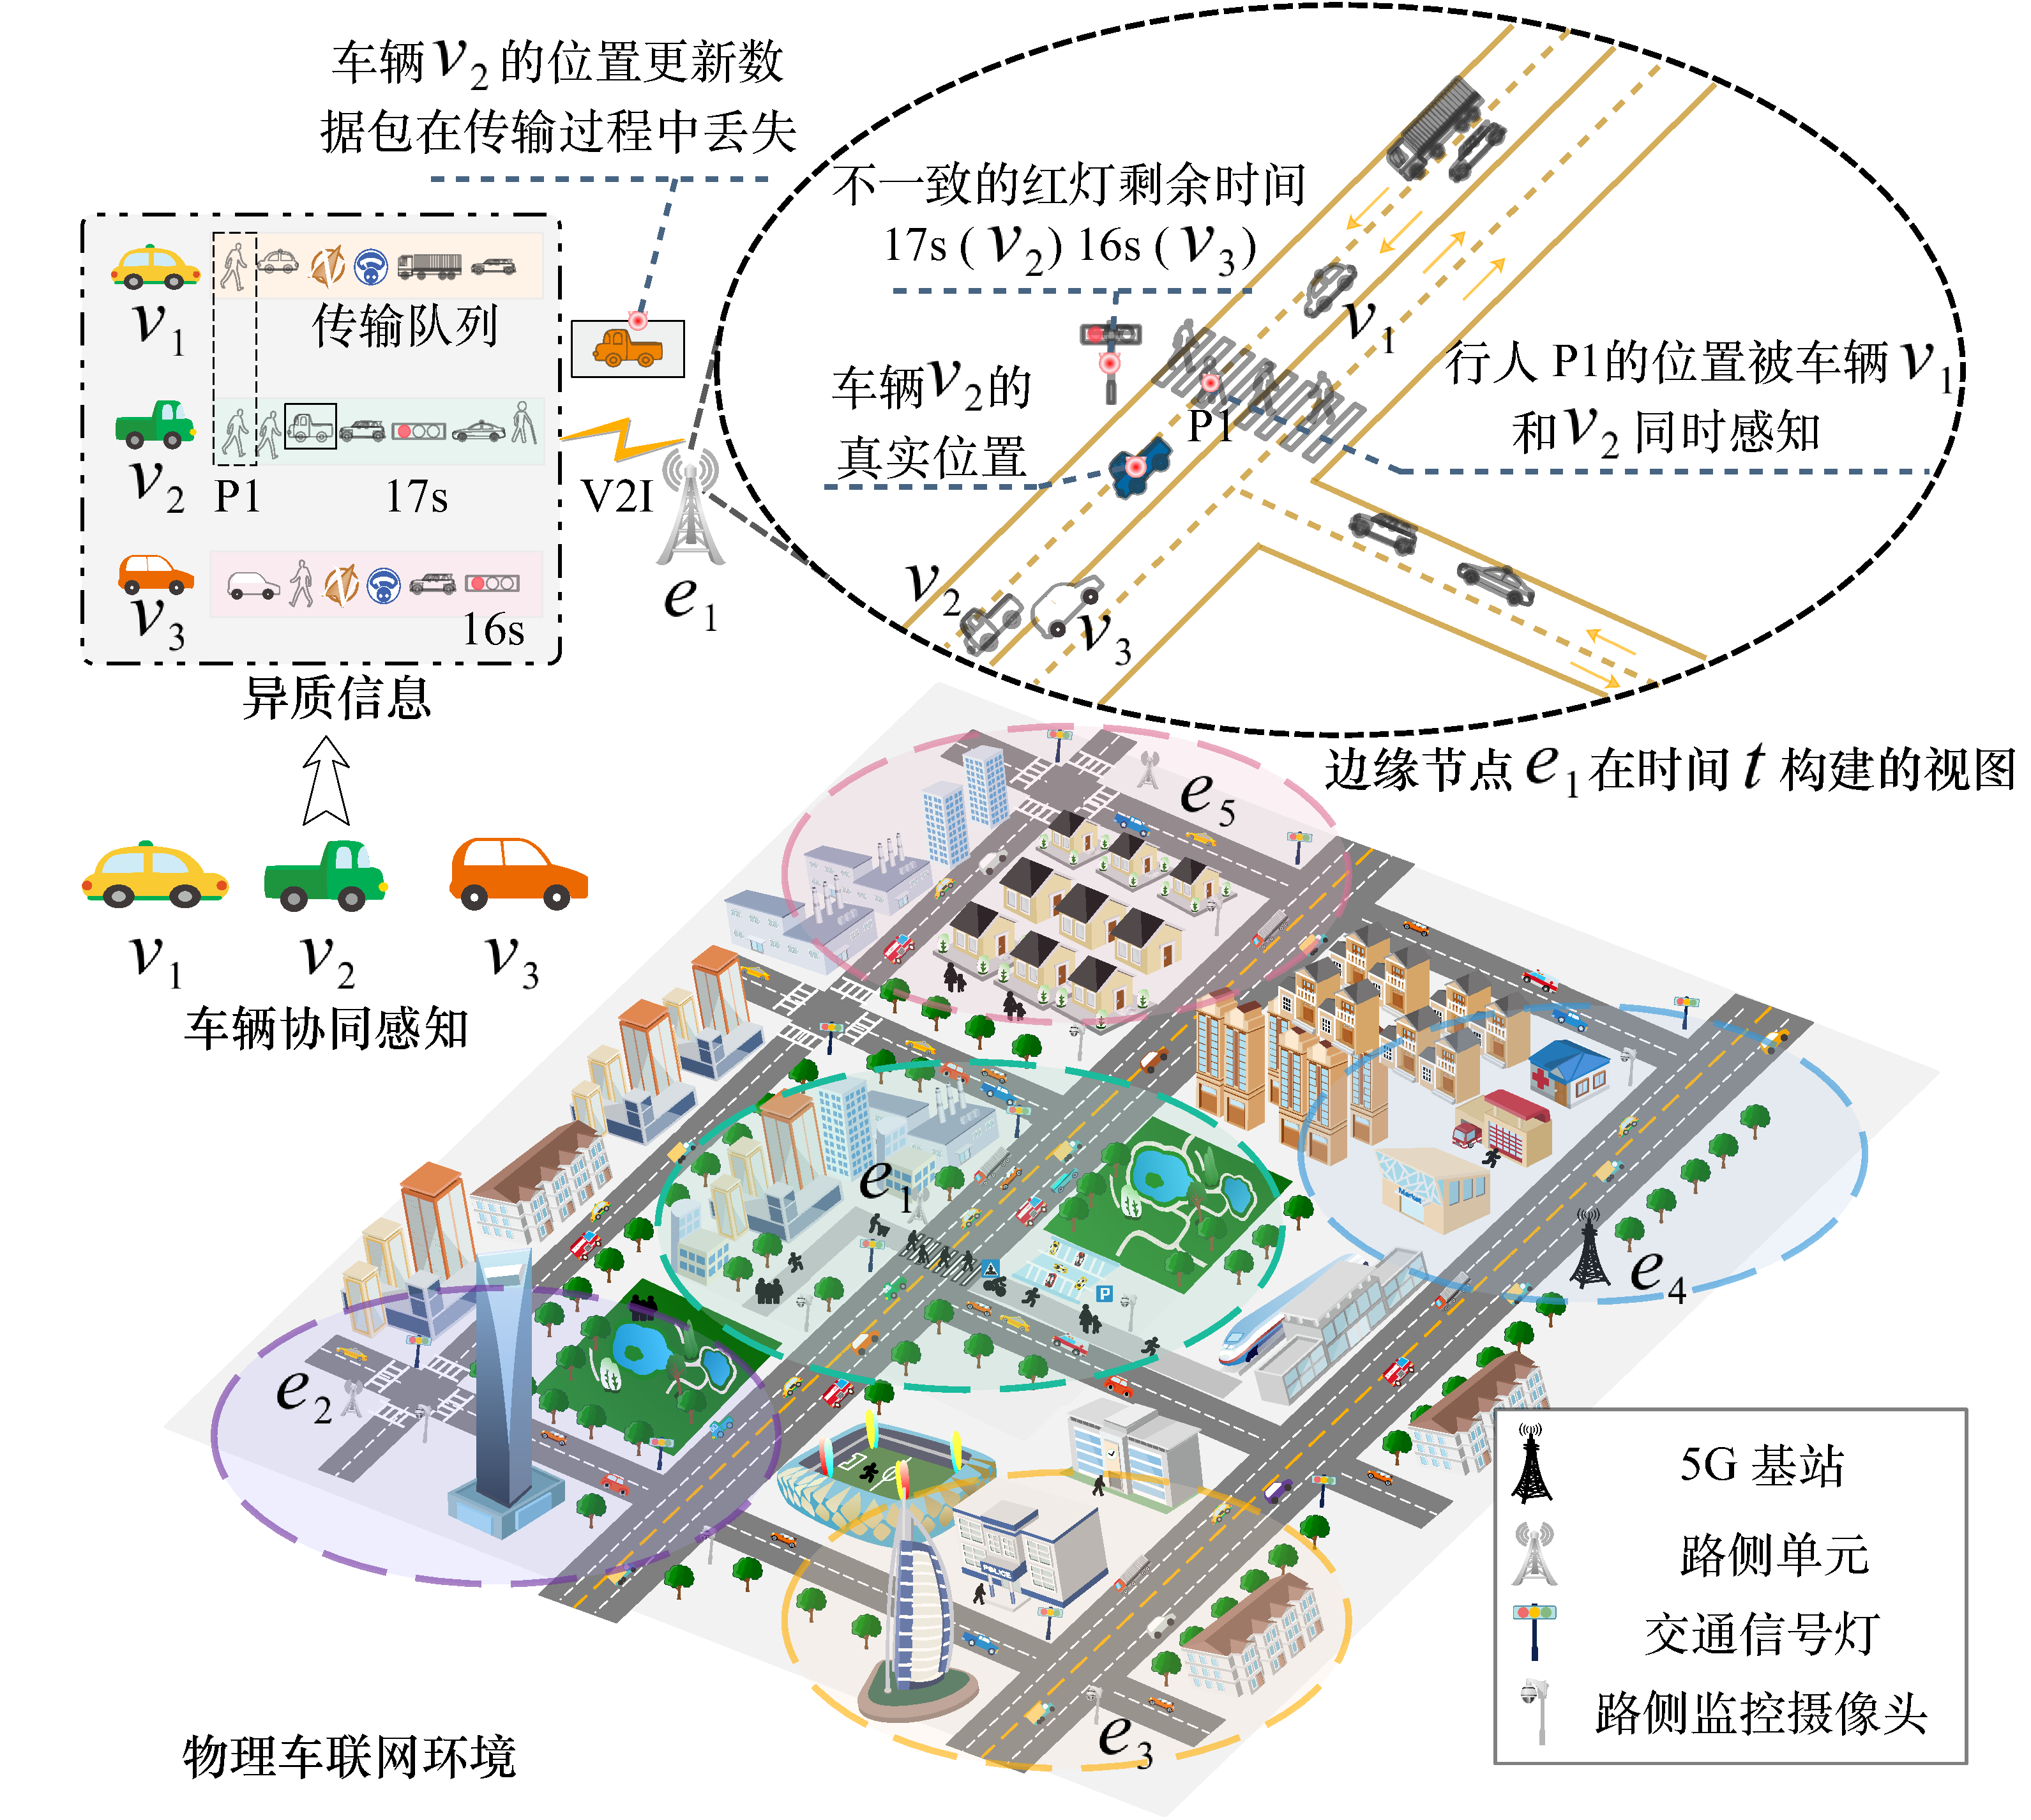
\includegraphics[width=0.65\columnwidth]{Fig3-1a-architerture.pdf}}
     \subfloat[][]{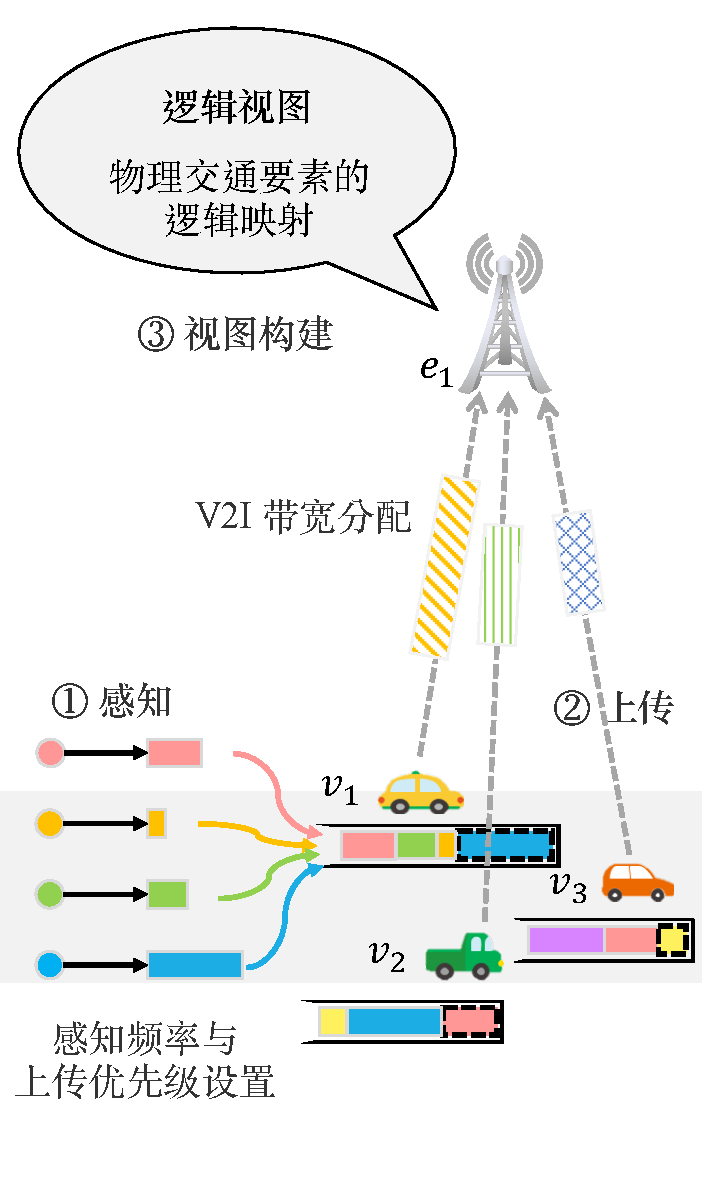
\includegraphics[width=0.35\columnwidth]{Fig3-1b-procedures.pdf}}
     \bicaption[系统架构]{系统架构。(a) 车载信息物理融合系统中合作传感和异质信息融合 (b) 系统工作流程}[System architecture]{System architecture. (a) Cooperative sensing and heterogeneous information fusion in VCPS (b) System workflow}
     \label{fig 3-1}
\end{figure}

本章节介绍了VCPS面向车载边缘计算的协作感知和异质信息融合架构。
如图\ref{fig 3-1}(a)所示,本架构可分为两个层次:物理车联网环境和由边缘节点构建的逻辑视图。
特别地,5G基站和路侧单元(如$e_1$$\sim$$e_5$)作为边缘节点被安装在道路旁边提供服务。
车辆能够在无线电覆盖范围内通过V2I通信与边缘节点进行通信,并通过搭载的车载传感器(例如LiDAR、GPS和相机)感知异质信息。
显然,车联网中的物理信息具有高度的动态性和时空相关性。
同时,搭载传感器的车辆具有异质性能力和有限资源,车联网通信也具有间歇性和不可靠性。
因此,关键在于要有一个量身定制的指标来定量评估由边缘节点构建的逻辑视图的质量,从而有效地衡量VCPS的整体性能。

本系统的工作流程如图\ref{fig 3-1}(b)所示,边缘节点$e_1$的逻辑视图构建包括三个步骤。
步骤1(感知):每辆车都可能根据其位置和感知能力感知到不同的信息。
被感知的信息在每辆车上排队,以便上传到边缘节点,每辆车将决定这些信息的感知频率和上传优先级。
步骤2(上传):边缘节点将V2I带宽(即不同范围的非重叠频谱)分配给有上传任务的车辆,以便这些车辆能够同时上传他们的传感信息而不受干扰。
步骤3(视图构建):边缘节点根据具体的ITS应用要求,将收到的物理信息映射到相应的逻辑元素上,从而构建逻辑视图。

本系统的特点总结如下。
首先,异质信息由车辆以不同的感知频率感知,因此不同信息的到达时刻可能不同。
提高感知频率可以提高信息的新鲜度,但也会延长排队延迟。
其次,必须综合考虑信息的不同数据量、V2I通信的连接性和视图要求,确定不同信息的上传优先级。
再次,由于边缘节点的带宽资源有限且车辆信道条件多变,分配的V2I带宽可能不足以支持及时上传数据。
因此,将更大的带宽分配给准备上传更新鲜、更紧急信息的车辆,而不是在更差的信道条件下(如离开V2I覆盖范围),以最大化带宽效率是有意义的。
最后,通过对车辆和边缘节点之间的信噪比(SNR)建模来考虑了不同车辆的信道条件,同时,V2I传输速率由两个节点之间的距离和分配的带宽决定。

此外,本章提供了一个例子来更好地说明上述观点。
如图\ref{fig 3-1}(a)所示,在$t$时间,边缘节点$e_1$构建了一个逻辑视图,根据车辆$v_1$、$v_2$和$v_3$感知和上传的信息,在交叉路口启用了速度建议应用。
通常,这种应用的目标是向正在接近交叉口的车辆提供最佳速度建议,使车辆可以顺利通过,从而达到最大化的整体交通效率。
假设车辆$v_2$和$v_3$都能感知交通灯信息,但感知的红灯剩余时间数值不一致。
例如,车辆$v_2$观察到红灯剩余17秒,而$v_3$观察到16秒,导致信息不一致。
另外,需要注意的是,同一物理要素的状态(例如行人P1的位置)可能会被多辆车(例如车辆$v_1$和$v_2$)同时感知到。
在这种情况下,它只需要由其中一辆车(例如车辆$v_1$)在一定时间内上传以节省V2I带宽。
只要物理要素在边缘节点以相同的质量水平建模,它就可以应用于不同的应用,而不需要由不同的车辆重复上传。
此外,数据包丢失可能导致物理车联网环境和视图之间的差距。
例如,假设车辆$v_2$的位置更新数据包丢失,这会导致其真实位置与$t$时间视图上的模型位置之间存在明显的不一致。
如上所述,定量测量边缘节点构建的视图的质量,并为协作感知和信息融合设计有效的调度机制,以最大限度地提高VCPS的整体质量是至关重要且具有挑战性的。

\section{指标设计}\label{section 3-3}

\subsection{基本符号}

系统的离散时间片集合用$\mathbf{T}=\{1, \ldots, t, \ldots, T\}$表示,其中$T$是时间片的数量。
异质信息的集合用$\mathbf{D}=\{1, \ldots, d, \ldots, D\}$表示。
信息集合$\mathbf{D}$中信息$d$可以用一个双元组$d=\left(\operatorname{type}_d, \left|d\right| \right)$表示,其中$\operatorname{type}_d$为类型,$\left|d\right|$为数据量。
车辆的集合用$\mathbf{V}=\{1, \ldots, v, \ldots, V\}$表示。
车辆集合$\mathbf{V}$中车辆$v$的特征用一个三元组$v=\left (l_v^t, \mathbf{D}_v, \pi_v \right )$表示,其中$l_v^t$是车辆$v$在时间$t$的位置;$\mathbf{D}_v$是车辆$v$可以感知的信息集合,$\pi_v$是车辆$v$的传输功率。
边缘节点的集合用$\mathbf{E}=\{1, \ldots, e, \ldots, E\}$表示。
边缘节点集合$\mathbf{E}$中边缘节点$e$的特征用一个三元组$e=\left (l_e, g_e, b_e \right)$表示,其中$l_e$是位置,$g_e$是通信范围,$b_e$是带宽。
车辆$v$与边缘节点$e$在时间$t$上的距离用$\operatorname{dis}_{v,e}^t \triangleq \operatorname{distance} \left (l_v^t, l_e \right ), \forall v \in \mathbf{V}, \forall e \in \mathbf{E}, \forall t \in \mathbf{T}$表示,其中$\operatorname{distance}\left(\cdot,\cdot\right)$是欧氏距离。

车辆$v$在$t$时间所感知的信息集合用$\mathbf{D}_v^t\subseteq \mathbf{D}_v$表示。
对于$\mathbf{D}_v^t$中的任意信息$d$,信息类型都是不同的,即$\operatorname{type}_{d^*} \neq \operatorname{type}_{d}, \forall d^* \in \mathbf{D}_v^t \setminus \left\{ d\right \}, \forall d \in \mathbf{D}_v^t$。
车辆$v$在时间$t$对于信息$d$的感知频率用$\lambda_{d,v}^t$表示。
由于感知能力有限,车辆感知频率需满足$\lambda_{d,v}^{t} \in [\lambda_{d,v}^{\min} , \lambda_{d,v}^{\max} ], \forall d \in \mathbf{D}_v^t, \forall v \in \mathbf{V}, \forall t \in \mathbf{T}$, 其中 $\lambda_{d,v}^{\min}$ 和 $\lambda_{d,v}^{\max}$ 分别为车辆$v$对于类型为$\operatorname{type}_{d}$的信息的最低和最高感知频率。
车辆$v$中的信息$d$在时间$t$的上传优先级用$p_{d,v}^t$表示,且${p}_{d^*, v}^t \neq {p}_{d, v}^t, \forall d^* \in \mathbf{D}_v^t \setminus \left\{ d\right \}, \forall d \in \mathbf{D}_v^t, \forall v \in \mathbf{V}, \forall t \in \mathbf{T}$。
在$t$时间内处于边缘节点$e$的无线电覆盖范围内的车辆集合表示为$\mathbf{V}_e^t=\left \{v \vert \operatorname{dis}_{v,e}^t \leq g_e, \forall v \in \mathbf{V} \right \}, \mathbf{V}_e^t \subseteq \mathbf{V}, \forall e \in \mathbf{E}$。
边缘节点$e$在时间$t$为车辆$v$分配的V2I带宽用$b_{v, e}^t$表示,且$b_{v, e}^t \in \left [0,b_e \right], \forall v \in \mathbf{V}_e^{t}, \forall e \in \mathbf{E}, \forall t \in \mathbf{T}$。
边缘节点$e$分配的V2I带宽之和不能超过其容量$b_e$,即,${\sum_{\forall v \in \mathbf{V}_e^{t}}b_{v, e}^t} \leq b_e, \forall e \in \mathbf{E}, \forall t \in \mathbf{T}$。

\subsection{系统模型}
本系统协同感知模型如图\ref{fig 3-2}所示。
车辆感知的信息到达间时间和排队时间通过利用多类M/G/1优先级队列(Multi-Class M/G/1 Priority Queue)\cite{qian2020minimizing}对车辆中的感知信息队列进行建模得到。
假定车辆$v$中具有相同类型$\operatorname{type}_d$的信息传输时间分布在每个时隙内保持稳定。
类型为$\operatorname{type}_d$的信息传输时间$\operatorname{\hat{g}}_{d, v, e}^t$遵循一类一般分布(General Distribution),其均值为$\alpha_{d, v}^t$,二阶矩和三阶矩分别为$\beta_{d, v}^t$和$\gamma_{d, v}^t$,那么该分布集合可以表示为
\begin{align}
	\mathbb{P}=\left\{\hat{\mathrm{g}}_{d, v, e}^t:\right. & \mathbb{E}\left[\hat{\mathrm{g}}_{d, v, e}^t\right]=\alpha_{d, v}^t, \notag \\
	& \mathbb{E}\left[\hat{\mathrm{g}}_{d, v, e}^t-\alpha_{d, v}^t\right]^2=\beta_{d, v}^t \notag \\
	& \mathbb{E}\left[\operatorname{\hat{g}}_{d, v, e}^t-\alpha_{d, v}^t\right]^{3}=\left.\gamma_{d, v}^t \right\}
\end{align}
因此,上传负载 $\rho_{v}^{t}$ 可表示为 
\begin{equation}
    \rho_{v}^{t}=\sum_{\forall d \subseteq \mathbf{D}_v^t} \lambda_{d,v}^{t}  \alpha_{d, v}^t
\end{equation}

\begin{figure}[h]
\centering
  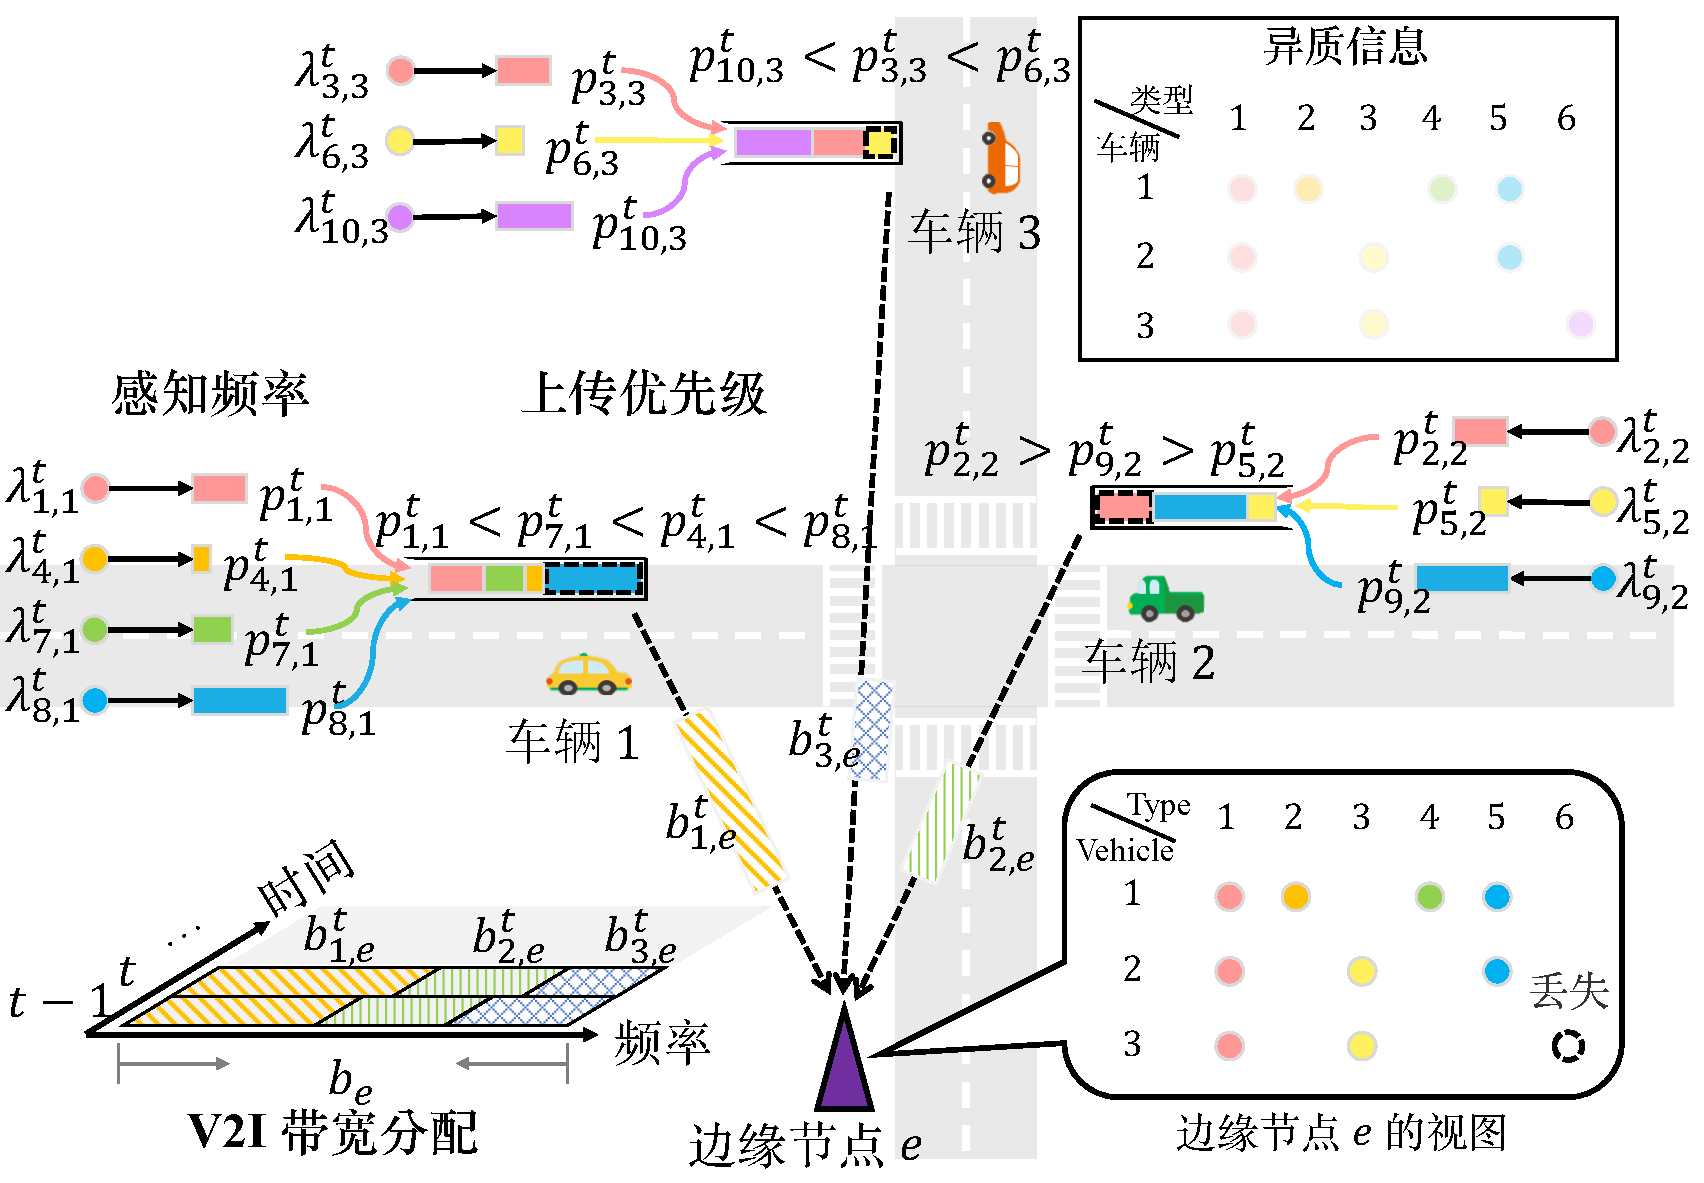
\includegraphics[width=1\columnwidth]{Fig3-2-cooperative-sensing.pdf}
  \bicaption{协同感知模型}{Cooperative sensing model}
  \label{fig 3-2}
\end{figure}

为了确保队列具有稳定状态, 需要满足 $\rho_{v}^{t} < 1$.
到达间隔时间$\operatorname{a}_{d, v}^t$是指车辆$v$中两个相邻的具有相同类型$\operatorname{type}_d$的信息到达时间差,其计算公式为  
\begin{equation}
    \operatorname{a}_{d, v}^t=\frac{1}{\lambda_{d, v}^{t}}
\end{equation}
在$t$时间内,车辆$v$中比信息$d$有更高上传优先权的信息集合被表示为
\begin{equation}
\mathbf{D}_{d, v}^t=\left\{d^* \mid p_{d^*, v}^t>p_{d, v}^t, \forall d^* \in \mathbf{D}_v^t\right\} 
\end{equation}
其中$p_{d^*, v}$是信息$d^* \in \mathbf{D}_v^t$的上传优先级。
  因此,信息$d$前面的上传负载(即车辆$v$在$t$时间内要在$d$前面上传的数据量)表示为
\begin{equation}
\rho_{d, v}^t=\sum_{\forall d^* \in \mathbf{D}_{d, v}^t} \lambda_{d^*, v}^t \alpha_{d^*, v}^t
\end{equation}
其中$\lambda_{d^*, v}^t$和$\alpha_{d^*, v}^t$分别是$t$时间内车辆$v$中信息$d^*$的感知频率和平均传输时间。
车辆$v$中类型为$\operatorname{type}_d$的信息的排队时间用$\operatorname{q}_{d, v}^t$表示。
根据Pollaczek$-$Khintchine公式\cite{takine2001queue},平均排队时间$\operatorname{\bar{q}}_{d, v}^t$计算如下。
\begin{equation}
    \operatorname{\bar{q}}_{d, v}^t= \frac{1} {1 - \rho_{d, v}^{t}} 
        \left[ \alpha_{d, v}^t + \frac{ \lambda_{d, v}^{t} \beta_{d, v}^t + \sum\limits_{\forall d^* \in \mathbf{D}_{d, v}^t} \lambda_{d^*,s}^t \beta_{d^*, v}^t }{2\left(1-\rho_{d, v}^{t} - \lambda_{d, v}^{t}  \alpha_{d, v}^t\right)}\right] 
        - \alpha_{d, v}^t
\label{equ 3-6}
\end{equation}
排队时延分析见附录\ref{appendix e}。

进一步,本章根据香农理论对通过V2I通信的数据上传进行建模。
车辆$v$和边缘节点$e$之间在时间$t$的V2I通信的信噪比(Signal-to-Noise Ratio,简称 SNR)用$\operatorname{SNR}_{v, e}^{t}$表示,其计算方法是\cite{sadek2009distributed}
\begin{equation}
    \label{equ 3-7}
    \operatorname{SNR}_{v, e}^{t}=\frac{1}{N_{0}}  \left|h_{v, e}\right|^{2} \zeta  {\operatorname{dis}_{v, e}^{t}}^{-\varphi} {\pi}_v
\end{equation}
其中$N_{0}$为加性白高斯噪声(Additive White Gaussian Noise,简称 AWGN);$h_{s, e}$为信道衰减增益;$\zeta$为常数,取决于天线设计,$\varphi$为路径损耗指数。
然后,车辆$v$和边缘节点$e$之间在时间$t$的V2I传输率,用$\operatorname{z}_{v, e}^t$表示,计算如下 
\begin{equation}
    \operatorname{z}_{v, e}^t=b_{v, e}^{t} \log _{2}\left(1+\mathrm{SNR}_{v, e}^{t}\right)
    \label{equ 3-8}
\end{equation}
其中$b_{v, e}^{t}$是分配给车辆$v$在时间$t$的带宽。
值得注意的是,给定车辆$v$的传输功率$\pi_s$,车辆$v$和边缘节点$e$之间在时间$t$的V2I通信的信噪比可以通过公式\ref{equ 3-7}得到,进一步可由公式\ref{equ 3-8}得到传输速率。
因此,信息$d$从车辆$v$到边缘节点$e$的传输时间用$\mathrm{w}_{d, v, e}^t$表示,其计算公式为
\begin{equation}
	\mathrm{w}_{d, v, e}^t=\frac{\left|d\right|}{\operatorname{z}_{v, e}^t}
\end{equation}
成功传输需要在数据包传输过程中,接收到的信噪比高于某个阈值,其被称为信噪比墙(SNR Wall)\cite{tandra2008snr},该阈值通过以下方式获得 
\begin{equation}
\mathrm{SNR}_{\text {wall }}=\frac{\sigma^{2}-1}{\sigma}
\end{equation}
其中$\sigma=10^{\nu / 10}$,$\nu$是以dB衡量的参数,量化了噪声不确定性的大小,且$\left(\nu^2 - 1\right) {N_0} = {\pi_v} \nu $。
因此,表示信息$d$是否从车辆$v$成功传输到边缘节点$e$的成功传输指标可表示为 
\begin{numcases}{\operatorname{c}_{d, v, e}^t=}
1, \forall {t^{*}} \in\left[t + \operatorname{\bar{q}}_{d, v}^t, t + \operatorname{\bar{q}}_{d, v}^t + \operatorname{w}_{d, v, e}^t\right], \operatorname{SNR}_{v, e}^{t^{*}}>\mathrm{SNR}_{\text {wall }} \notag \\
0, \exists {t^{*}} \in\left[t + \operatorname{\bar{q}}_{d, v}^t, t + \operatorname{\bar{q}}_{d, v}^t + \operatorname{w}_{d, v, e}^t\right], \operatorname{SNR}_{v, e}^{t^{*}} \leq \mathrm{SNR}_{\text {wall }}
\end{numcases}
因此,由车辆$v$传输并由边缘节点$e$接收的信息集合表示为 $\mathbf{D}_{v, e}^t = \{ d \mid \operatorname{c}_{d, v, e}^t = 1, \forall d \in \mathbf{D}_v \}, \mathbf{D}_{v, e}^t \subseteq \mathbf{D}_v^t, \forall v \in \mathbf{V}, \forall e \in \mathbf{E}$.


\subsection{Age of View}
系统中的视图集合用$\mathbf{I}$表示,视图$i \in \mathbf{I}$所需的信息集用$\mathbf{D}_{i}$表示,它是特定ITS应用所需的物理交通元素的映射,它表示为
\begin{equation}
	\mathbf{D}_{i} = \{d \mid y_{d, i} = 1, \forall d \in \mathbf{D} \}
\end{equation}
视图$i$所需元素的数量用$|\mathbf{D}_{i}|$表示。
边缘节点$e$在$t$时间所需的视图集合用$\mathbf{I}_e^t \subseteq \mathbf{I}$表示。
因此,边缘节点$e$收到的并被视图$i$需要的信息集用以下方式表示
\begin{equation}
    \mathbf{D}_{i, e}=\bigcup_{\forall i \in \mathbf{I}}\left(\mathbf{D}_i \cap \mathbf{D}_{v, e}^t\right), \forall v \in \mathbf{V}_e^t, \forall e \in \mathbf{E}
\end{equation}
和$| \mathbf{D}_{i, e} |$是边缘节点$e$收到并被视图$i$需要的信息数量。
然后,本章定义了异质信息融合的三个特征,包括视图的及时性、完整性和一致性,如下所示。

首先,异质信息是随时间变化的,信息的新鲜度对于建立视图的质量模型至关重要。
因此,本章对车辆$v$中的信息$d$的时效性定义如下。
\begin{definition}[\textbf{信息 $d$的时效性}]
	车辆$v$的信息$d$的时效性 $\xi_{d,v} \in (0, +\infty)$被定义为信息$d$的间隔到达时间、排队时间和传输时间之和。
	\begin{equation}
    	\xi_{d, v} = \operatorname{a}_{d, v}^t + \operatorname{q}_{d, v}^t + \operatorname{w}_{d, v, e}^t, \forall d \in \mathbf{D}_v^t, \forall v \in \mathbf{V}
	\end{equation}
\end{definition}
\noindent 其中 $\operatorname{a}_{d, v}^t$、$\operatorname{q}_{d, v}^t$ 和 $\operatorname{w}_{d, v, e}^t$ 分别为信息$d$的间隔到达时间、排队时间和传输时间。
因此,视图的时效性定义如下。
\begin{definition}[\textbf{视图$i$的时效性}]
视图$i$的时效性 $\Xi_{i} \in (0,+\infty)$被定义为信息实效性之和。
	\begin{equation}
    	\Xi_{i} = \sum_{\forall v \in \mathbf{V}} \sum_{\forall d \in \mathbf{D}_{i, e} \cap \mathbf{D}_v^t } \xi_{d, v}, \forall i \in \mathbf{I}_e^t, \forall e \in \mathbf{E}
	\end{equation}
\end{definition}

其次,车联网具有包括车辆的高流动性、有限的网络资源和不可靠的无线通信的固有特性。
由于车辆和边缘节点之间的无线传输连接断开,或者传输过程中数据包的丢失,视图可能是不完整的。
因此,本章对视图的完整性定义如下。
\begin{definition}[\textbf{视图$i$的完整性}]
	视图$i$的完整性$\Phi_{i} \in [0,1]$被定义为边缘节点$e$实际收到的信息数量与所需总量之比。
	\begin{equation}
	\Phi_{i}= {| \mathbf{D}_{i, e} |} \big/ {|D_{i} |}, \forall i \in \mathbf{I}_e^t, \forall e \in \mathbf{E}
	\end{equation}
\end{definition}
\noindent 其中$|\mathbf{D}_{i, e}|$是边缘节点$e$收到并被视图$i$需要的信息数,$|\mathbf{D}_{i}|$是视图$i$需要的信息总数。

第三,由于不同类型的信息有各自的感知频率和上传优先级,在构建视图时,必须使不同类型信息的版本尽可能接近。
因此,本章对视图的一致性定义如下。 
\begin{definition}[\textbf{视图$i$的一致性}]
视图$i$的一致性$\Psi_{i} \in (0,+\infty)$被定义为信息接收时间与视图所需信息的平均接收时间之差的二次方和。
\begin{equation}
\Psi_{i}=\sum_{\forall v \in \mathbf{V}} \sum_{\forall d \in \mathbf{D}_{i, e} \cap \mathbf{D}_v^t} \left|\operatorname{q}_{d, v}^t + \operatorname{w}_{d, v, e}^t - \psi_{i} \right|^{2}, \forall i \in \mathbf{I}_e^t, \forall e \in \mathbf{E}
\end{equation}
\end{definition}
\noindent 其中 $\psi_{i}$ 是视图$i$所需信息的平均接收时间,其可由下式得到 
\begin{equation}
	\psi_{i} = \frac{1}{|D_{i, e}|} {\sum_{\forall v \in \mathbf{V}}\sum_{\forall d \in D_{i, e} \cap \mathbf{D}_v^t} \left( \operatorname{q}_{d, v}^t + \operatorname{w}_{d, v, e}^t\right) }, \forall i \in\mathbf{I}_e^t, \forall e \in \mathbf{E}
\end{equation}

最后,本章给出了Age of View的正式定义,它综合了视图的及时性、完整性和一致性。
\begin{definition}[\textbf{Age of View, AoV}]
Age of View $\operatorname{AoV}_{i} \in (0, 1)$ 被定义为视图$i$的归一化及时性、完整性和一致性的加权平均数。
	\begin{equation}
	    \operatorname{AoV}_{i} = w_1  \hat{\Xi}_{i} + w_2  \hat{\Phi}_{i}+  w_3 \hat{\Psi}_{i}, \forall i \in \mathbf{I}_e^t, \forall e \in \mathbf{E}
\end{equation}
\end{definition}
\noindent 其中,$\hat{\Xi}_{i} \in (0, 1)$,$\hat{\Phi}_{i} \in (0, 1)$和$\hat{\Psi}_{i} \in (0, 1)$分别表示视图$i$的归一化及时性、归一化完整性和归一化一致性。
需要注意的是,由于观点的及时性、完整性和一致性的维度不同,为了形成AoV的统一表示,根据最小-最大比例,将它们归一化为$(0,1)$,具体如下
\begin{numcases}{}
\hat{\Xi}_{i} = {\Xi}_{i} \big/ \left( \delta_\xi | \mathbf{D}_{v, e} |   T \right) \notag \\ 
\hat{\Phi}_{i} = 1 - {\Phi}_{i}  \notag \\
\hat{\Psi}_{i} = {\Psi}_{i} \big/ \left( \delta_\psi  \max\limits_{\substack{\forall d \in \mathbf{D}_v \cap \mathbf{D}_v^t \\ \forall v \in \mathbf{V}}}{\left\{ \left|\operatorname{q}_{d, v}^t + \operatorname{g}_{d, v, e}^t - \psi_{i} \right|^{2}\right\}}   \right)
\end{numcases}
\noindent 其中$\delta_{\xi} \in(0,1)$和$\delta_\psi \in(0,1)$分别是及时性和一致性的数据比例系数。它们被用来避免在最小-最大比例中通过缩减及时性和一致性的理论最大值将大部分数值集中在一个小范围内。

$\hat{\Xi}_{i}$、$\hat{\Phi}_{i}$和$\hat{\Psi}_{i}$的加权系数分别用$w_1$、$w_2$和$w_3$表示,且$w_1+w_2+w_3=1$。
这三个加权系数可以根据ITS应用的不同要求进行相应的调整。
例如,对于道路交叉口的速度咨询应用,车辆需要从边缘节点接收实时速度的指令,以便安全顺利地通过交叉口。在这种情况下,及时性因素(例如,实时交通灯状态)与完整性因素(例如,行人在视图中被建模)相比,在视图中被建模更为重要。
请注意,$\operatorname{AoV}_{i}$的值越低,说明构建的视图质量越高。

\subsection{问题定义}
鉴于上述指标AoV是单独评估视图的质量,本章进一步在系统层面上定义VCPS的质量如下。
\begin{definition}[\textbf{VCPS 质量}]
VCPS的质量$\Upsilon \in (0,1)$被定义为在调度期$T$中边缘节点的每个视图$i$的AoV的平均值。
\begin{equation}
\Upsilon=\frac{\sum_{\forall t \in \mathbf{T}} \sum_{\forall e \in \mathbf{E}} \sum_{\forall i \in \mathbf{I}_e^t} \left(1 - \operatorname{AoV}_{i}\right)}{\sum_{\forall t \in \mathbf{T}} \sum_{\forall e \in \mathbf{E}} |\mathbf{I}_e^t| }
\end{equation}
\end{definition}

给定一个解决方案$(\bf\Lambda, \mathbf{P}, \mathbf{B} )$,其中$\bf\Lambda$表示确定的感知频率,$\mathbf{P}$表示确定的上传优先级,$\mathbf{B}$表示确定的V2I带宽分配,它们分别表示为 
\begin{numcases}{}
\bf\Lambda = \left \{ \lambda_{d,v}^{t} \vert \forall d \in \mathbf{D}_v^t  , \forall v \in \mathbf{V}, \forall t \in \mathbf{T} \right \} \notag \\ 
\mathbf{P} = \left \{ p_{d,s}^{t} \vert \forall d \in \mathbf{D}_v^t  , \forall v \in \mathbf{V}, \forall t \in \mathbf{T}\right \} \notag \\
\mathbf{B} = \left \{ b_{v, e}^t \vert \forall v \in \mathbf{V}_e^t, \forall e \in \mathbf{E}, \forall t \in \mathbf{T}\right \}
\end{numcases}
\noindent 本章节的目标问题是通过确定感知频率、上传优先级,以及V2I带宽,以最大限度地提高VCPS的质量,其形式化定义如下。
\begin{align}
	&\max_{\bf\Lambda, \mathbf{P}, \mathbf{B}} \Upsilon \notag \\
	\text { s.t. }
    \mathcal{C}3.1: & \lambda_{d,v}^{t} \in \left [\lambda_{d,v}^{\min} , \lambda_{d,v}^{\max} \right ], \forall d \in \mathbf{D}_v^t , \forall v \in \mathbf{V}, \forall t \in \mathbf{T} \notag \\
     \mathcal{C}3.2: &{p}_{d^*, v}^t \neq {p}_{d, v}^t, \forall d^* \in \mathbf{D}_v^t \setminus \left\{ d\right \}, \forall d \in \mathbf{D}_v^t, \forall v \in \mathbf{V}, \forall t \in \mathbf{T} \notag \\
    \mathcal{C}3.3: & b_{v, e}^t \in \left[ 0 , b_e \right ], \forall v \in \mathbf{V}_e^t, \forall e \in \mathbf{E}, \forall t \in \mathbf{T} \notag \\
    \mathcal{C}3.4: & \sum_{\forall d \subseteq \mathbf{D}_v^t} \lambda_{d,v}^{t}  \alpha_{d, v}^t < 1,\ \forall v \in \mathbf{V}, \forall t \in \mathbf{T}  \notag \\
    \mathcal{C}3.5: & {\sum_{\forall v \in \mathbf{V}_e^{t}}b_{v, e}^t} \leq b_e, \forall e \in \mathbf{E}, \forall t \in \mathbf{T}
\end{align}


约束条件$\mathcal{C}3.1$要求车辆$v$中的信息$d$在$t$时间的感知频率应满足其感知能力的要求。
$\mathcal{C}3.2$ 保证$t$时间内车辆$v$中信息$d$的上传优先权。
$\mathcal{C}3.3$ 规定边缘节点$e$在$t$时间为车辆$v$分配的V2I带宽不能超过其带宽容量$b_e$。
$\mathcal{C}3.4$保证在调度周期$\mathbf{T}$内队列稳定状态。
$\mathcal{C}3.5$要求边缘节点$e$分配的V2I带宽之和不能超过其容量$b_e$。

\section{算法设计}\label{section 3-4}

\subsection{算法模型}
本章中,将详细介绍所提基于差分奖励的多智能体深度强化学习(Multi-Agent Difference-Reward-Based Deep Reinforcement Learning,简称 MDR)算法,其模型如图\ref{fig 3-3}所示,是由$V$辆车、边缘节点$e$、VCPS环境和经验回放缓冲区组成。
首先,车辆$v$决定其动作$\boldsymbol{a}_{v}^{t}$,包括确定感知频率和上传优先级。
特别地,车辆$v$的行动者网络被用来生成其动作,其输入是对系统状态的局部观测$\boldsymbol{o}_{v}^{t}$。
车辆$v$的评论家网络被用来评估由相应行动者网络产生的动作。
第二,边缘节点$e$决定其动作$\boldsymbol{a}_{e}^{t}$,根据预测的车辆轨迹和视图要求,为其无线电覆盖范围内的车辆分配V2I带宽。
第三,环境根据动作$\{ \boldsymbol{a}_{1}^{t}, \ldots, \boldsymbol{a}_{\mathbf{V}}^{t}, \boldsymbol{a}_{e}^{t}\}$ 获得系统奖励,即边缘节点$e$在时间$t$实现的VCPS质量。
采用基于DR的信用分配,将系统奖励分为差分奖励$\{r_1^t, \ldots, r_{V}^t\}$,其中$r_v^t$被用来评估车辆$v$对视图构建的贡献。
第四,相关的交互经验,包括系统状态、车辆动作、差分奖励和下一个系统状态,都存储在经验回放缓冲区中,它们被用来训练车辆的行动者和评论家网络。
算法模型的主要组成部分设计如下。

\begin{figure}[h]
\centering
  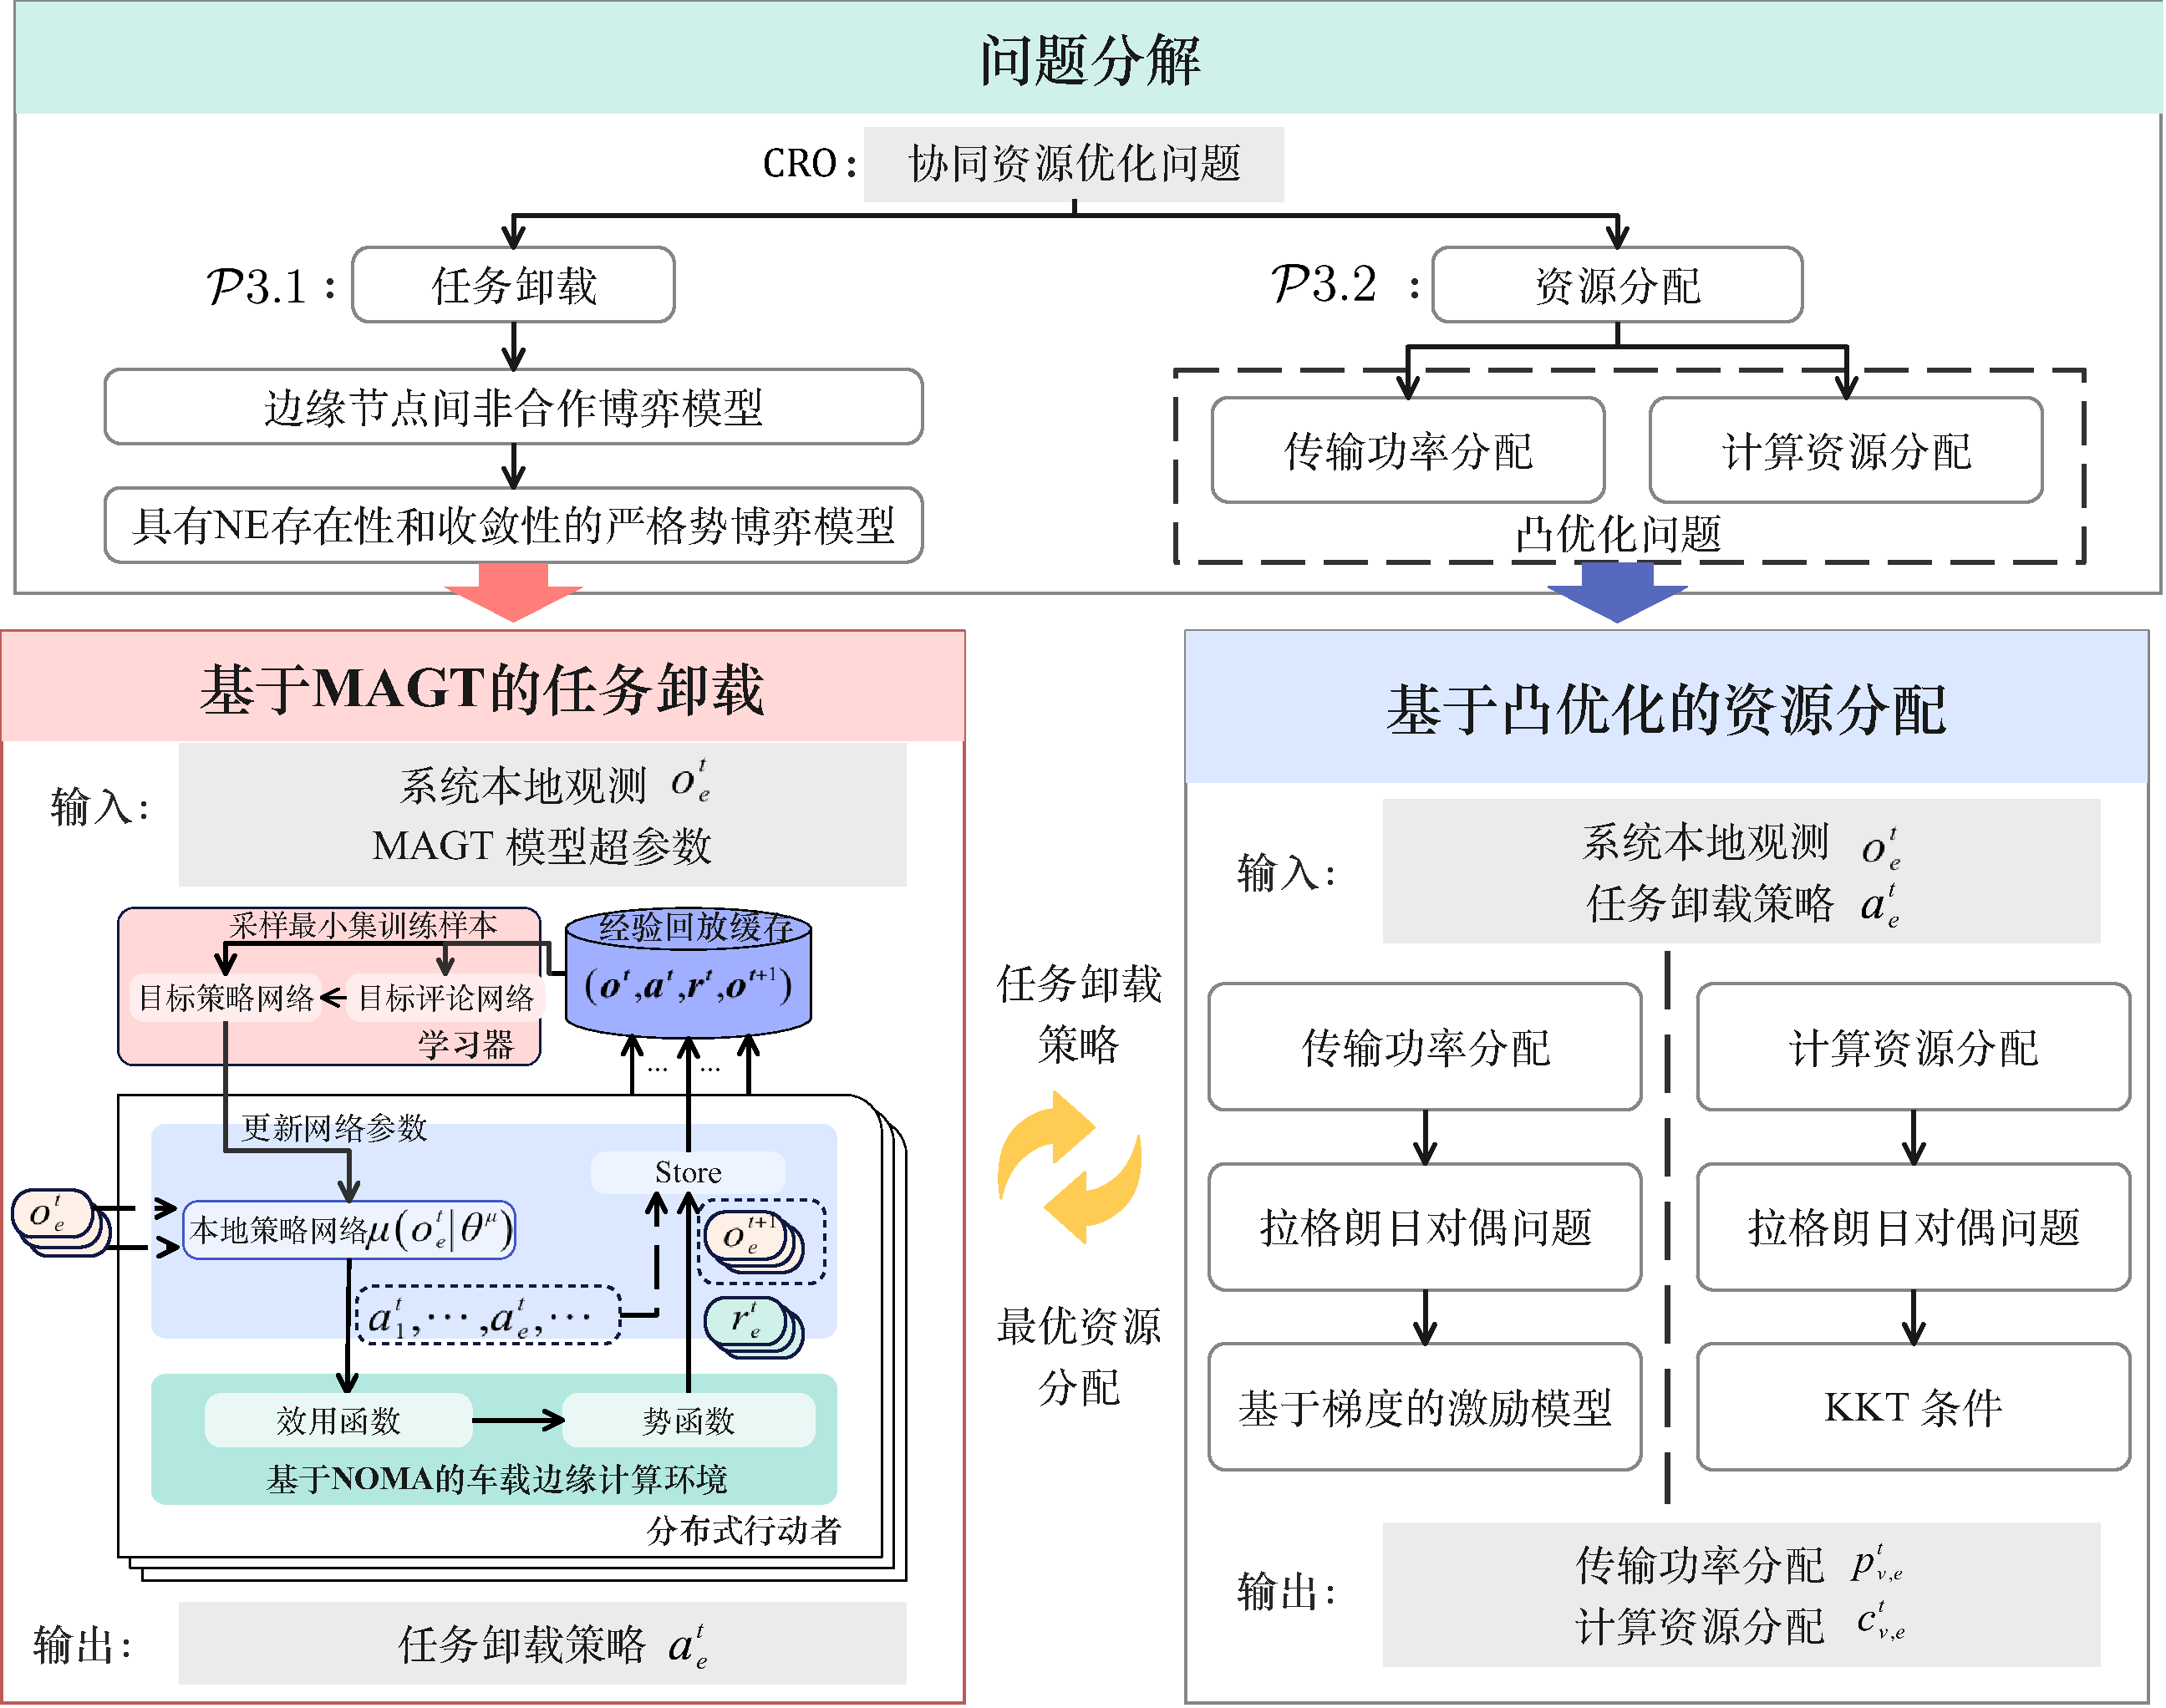
\includegraphics[width=1\columnwidth]{Fig3-3-solution-model.pdf}
  \bicaption{多智能体强化学习算法模型}{Multi-agent deep reinforcement learning model}
  \label{fig 3-3}
\end{figure}

1) \textbf{系统状态}: 边缘节点定期广播其视图需求和缓存信息。在$t$时间内,车辆$v$的系统状态的本地观测被表示为 
	\begin{equation}
		\boldsymbol{o}_{v}^{t}=\left\{\mathbf{D}_{v}^{t}, \mathbf{D}_{e}^{t}, \mathbf{I}_e^t\right\}
	\end{equation} 
	\noindent 其中$\mathbf{D}_{v}^{t}$代表车辆$v$在$t$时间感知的信息集合。
	$\mathbf{D}_{e}^{t}$ 代表$t$时边缘节点$e$中的缓存信息集合。
	和$\mathbf{I}_e^t$代表$e$在时间$t$的边缘节点所需的视图集合。
	时间$t$的系统状态被表示为:
	\begin{equation}
		\boldsymbol{o}^{t}=\left\{\mathbf{D}_{1}^{t}, \ldots, \mathbf{D}_{v}^{t}, \ldots, \mathbf{D}_{V}^{t}, \mathbf{D}_{e}^{t}, \mathbf{I}_{e}^{t}\right\}
	\end{equation}

2) \textbf{动作空间}: 车辆$v$的动作空间由$t$时间的感知频率和传感信息的上传优先级组成,它被表示为 
	\begin{equation}
		\boldsymbol{a}_{v}^{t}=\{ \lambda_{d, v}^{t}, p_{d, v}^{t} \mid \forall d \in \mathbf{D}_{s}^t\}
	\end{equation}
	\noindent 其中$\lambda_{d, v}^{t}$和$p_{d, v}^{t}$分别是$t$时间内车辆$v$中信息$d$的感知频率和上传优先级。
	车辆动作的集合用$\boldsymbol{a}_{\mathbf{V}}^{t} = \left\{\boldsymbol{a}_{v}^{t}\mid \forall v \in \mathbf{V}\right\}$表示。
	边缘节点的动作是对车辆进行V2I带宽分配,其表示为 
	\begin{equation}
		\boldsymbol{a}_{e}^{t}=\{b_{v, e}^{t} \mid \forall v \in \mathbf{V}_{e}^{t}\}
	\end{equation}
	其中$b_{v, e}^t$是边缘节点$e$在时间$t$为车辆$v$分配的V2I带宽。
	
3) \textbf{系统奖励}: 在系统状态$\boldsymbol{o}^{t}$下,通过车辆动作$\boldsymbol{a}_{\mathbf{V}}^{t}$和边缘节点动作$\boldsymbol{a}_{e}^{t}$的系统奖励被定义为$t$时边缘节点$e$实现的VCPS质量,其计算公式为
	\begin{equation}
		r\left(\boldsymbol{a}_{\mathbf{V}}^{t},\boldsymbol{a}_{e}^{t} \mid \boldsymbol{o}^{t}\right)=\frac{1}{\left|\mathbf{I}_e^t\right|} \sum_{\forall i \in \mathbf{I}_e^t}\left(1 -\operatorname{AoV}_{i} \right)
	\end{equation}
	
系统奖励展示了整个系统的综合表现,这表现来自于车辆和边缘节点的共同努力。
为了评估各车辆的贡献,需要将系统奖励分配给每个车辆作为个人奖励。
基于差分奖励(Difference Reward,简称DR)的信用分配方案是通过计算系统奖励与无该智能体动作所获奖励之间的差值来确定该智能体的个人奖励。
因此,可以更准确地评估每个智能体的行为,从而进一步提升所提出解决方案的性能。
据此,车辆$v$的差分奖励表示为\cite{foerster2018counterfactual}
\begin{equation}
r_{v}^{t}=r\left(\boldsymbol{a}_{\mathbf{V}}^{t},\boldsymbol{a}_{e}^{t} \mid \boldsymbol{o}^{t}\right)-r\left(\boldsymbol{a}_{\mathbf{V}-v}^{t},\boldsymbol{a}_{e}^{t} \mid \boldsymbol{o}^{t}\right)
\end{equation}
\noindent 其中 $r\left(\boldsymbol{a}_{\mathbf{V}-v}^{t},\boldsymbol{a}_{e}^{t} \mid \boldsymbol{o}^{t}\right)$是没有车辆$v$贡献的系统奖励,它可以通过设置车辆$v$的空动作集得到。
车辆的差分奖励集合用$\boldsymbol{r}_{\mathbf{V}}^{t}=\{ r_{v}^{t} \mid \forall v \in \mathbf{V}\}$表示。

\subsection{工作流程}
本算法包括三个部分,即初始化、回放经验存储和训练。

\SetKwInOut{KwIn}{输入}
\SetKwInOut{KwOut}{输出}

\begin{algorithm}[h]
\renewcommand{\algorithmcfname}{算法}
		\caption{基于差分奖励的多智能体深度强化学习(Multi-Agent Difference-Reward-Based Deep Reinforcement Learning,简称 MDR)}
		初始化网络参数\\
		初始化经验回放缓存$\mathcal{B}$\\
        \For{迭代次数 $= 1$ 到 最大迭代次数}{
            初始化一个随机过程 $\mathcal{N}$ 以进行探索 \\
            接收初始系统状态 $\boldsymbol{o}_{1}$\\
            \For{时间片 $t = 1$ 到 $T$}{
            	\For{车辆 $v=1$ 到 $V$ }{
            			接收本地观测值 $\boldsymbol{o}_{v}^{t}$ \\
                    	选择一个动作 $\boldsymbol{a}_{v}^{t}=\boldsymbol{\mu}_{v}\left(\boldsymbol{o}_{v}^{t} \mid \theta_{v}^{\mu}\right)+\mathcal{N}_{t}$ \\
            		得到所需信息 $\mathbf{D}_{v,\operatorname{R}}^{t}$\\
        		通过基于EM方法利用历史相对距离来预测移动模式\\
        		预测未来的轨迹 $\operatorname{Traj}_{v}^{t}$ \\
        		计算平均距离$\operatorname{\bar{dis}}_{v, e}^{t}$
            	}
        	\For{车辆 $v=1$ 到 $V$ }{
        		通过VBA策略分配带宽 $b_{v, e}^{t}$ 给车辆 $s$\\}
            	接收系统奖励 $r\left(\boldsymbol{a}_{\mathbf{V}}^{t},\boldsymbol{a}_{e}^{t} \mid \boldsymbol{o}^{t}\right)$ 和下一个系统状态 $\boldsymbol{o}^{t+1}$\\
            	划分系统奖励为差分奖励$\boldsymbol{r}_{\mathbf{V}}^{t}$\\
            	存储 $\left(\boldsymbol{o}^{t}, \boldsymbol{a}_{\mathbf{V}}^{t}, \boldsymbol{r}_{\mathbf{V}}^{t}, \boldsymbol{o}^{t+1}\right)$ 到经验回放缓存 $\mathcal{B}$
            }
            \For{车辆 $v=1$ 到 $V$ }{
            		从经验回放缓存$\mathcal{B}$随机采样 $M$ 训练样本\\
            		更新本地行动者和评论家网络参数\\
            	}
            	更新目标行动者和评论家网络参数
       	}
       	\label{algorithm 3-1}
\end{algorithm}

1) \textbf{初始化}: 每辆车都作为一个智能体由四个神经网络组成,即一个本地行动者网络、一个目标行动者网络、一个本地评论家网络和一个目标评论家网络。
车辆$v$的本地行动者和本地评价家网络的参数分别用$\theta_{v}^{\mu}$和$\theta_{v}^{Q}$来表示。
目标行动者和目标评论家网络的参数分别用$\theta_{v}^{\mu^{\prime}}$和$\theta_{v}^{Q^{\prime}}$表示。
车辆的本地行动者和本地评价家网络的参数是随机初始化的。
目标行动者和目标评论家网络的参数被初始化为与相应的本地网络相同。
\begin{align}
	\theta_{v}^{\mu^{\prime}} \leftarrow \theta_{v}^{\mu}, \forall v \in \mathbf{V}\\
	\theta_{v}^{Q^{\prime}} \leftarrow \theta_{v}^{Q}, \forall v \in \mathbf{V}
\end{align}
一个最大容量为$|\mathcal{B}|$的经验回放缓存被初始化,以存储车辆的回放经验。
该程序显示在算法3.1的第1-2行。

2) \textbf{回放经验存储}:
在每个迭代的开始,一个随机过程$\mathcal{N}$被初始化用于探索。
车辆$v$在时间$t$的行动是由本地行动者网络根据其对系统状态的本地观察得到的。
\begin{equation}
	\boldsymbol{a}_{v}^{t}=\boldsymbol{\mu}_{\boldsymbol{v}}\left(\boldsymbol{o}_{v}^{t} \mid \theta_{v}^{\mu}\right)+\mathcal{N}_{t}
\end{equation}
\noindent 其中,$\mathcal{N}_{t}$是一个探索噪音,以增加车辆动作的多样性。

边缘节点$e$根据预测的车辆轨迹和视图要求,通过VBA方案分配V2I带宽。
具体地说,首先,车辆的移动模式由边缘节点$e$根据车辆和边缘节点之间的历史距离,使用期望最大化(Expectation-Maximization,简称 EM)方法\cite{hofmann2001unsupervised} 进行预测。
然后,根据基于EM的移动性模式预测,预测车辆$v$在未来$H$时间片的轨迹,用$\operatorname{Traj}_{v}^{t} = \{ \hat{l}_{v}^{t+1}, \dots, \hat{l}_{v}^{t+h}, \dots, \hat{l}_{v}^{t+H}\}$表示,其中$\hat{l}_{v}^{t+h}$是车辆$v$在时间$t+h$的预测位置。
因此,车辆在边缘节点之间的平均距离是通过以下方式计算得到
\begin{equation}
	\operatorname{\bar{dis}}_{v, e}^{t} = \frac{1}{H} {\sum_{\forall h \in [1, H]} \widehat{\operatorname{dis}}_{v, e}^{t+h}}
\end{equation}
其中,$\widehat{\operatorname{dis}}_{v, e}^{t+h}$ 是车辆$v$预测位置与边缘节点的距离,而$\widehat{\operatorname{dis}}_{v, e}^{t+h}=\operatorname{distance}(\hat{l}_{v}^{t+h}, l_{e})$。

那么,由车辆$v$感知到的并被视图$i$在时间$t$所需的信息集表示为 
\begin{equation}
	\mathbf{D}_{v, i}^{t} = \left\{ d \mid  d \in \mathbf{D}_{v}^t \cap  \mathbf{D}_i \right\}
\end{equation}
因此,由车辆$v$感知到并被边缘节点$e$上所有视图在时间$t$所需的信息集合表示为 
\begin{equation}
	\mathbf{D}_{v, {\mathbf{I}_e^t}}^{t} = \{ d \mid  d \in \bigcup_{\forall v \in V_e^t} \mathbf{D}_{v, i}^{t}\}
\end{equation}
\noindent 该集合的大小记为$|\mathbf{D}_{v, {\mathbf{I}_e^t}}^{t}|$, 并可通过下式得到
\begin{equation}
	|\mathbf{D}_{v, {\mathbf{I}_e^t}}^{t}| = \sum_{\forall d \in \mathbf{D}_{v, {\mathbf{I}_e^t}}^{t}}|d|
\end{equation}
最后,边缘节点$e$为车辆$v$分配的V2I带宽由以下方式计算 
\begin{equation}
	b_{v, e}^{t} =\frac{b_{e}} {\omega+\operatorname{rank}_{v}}
\end{equation}
\noindent 其中$\omega$为常数,$\operatorname{rank}_{v}$为车辆$v$按$| \mathbf{D}_{v, {\mathbf{I}_e^t}}^{t}|$的序列降序并按$\operatorname{\bar{dis}}_{v, e}^{t}$的序列生序排列的排序。

在确定车辆和边缘节点的联合动作后,以实现的VCPS质量作为系统奖励$r\left(\boldsymbol{a}_{\mathbf{V}}^{t},\boldsymbol{a}_{e}^{t} \mid \boldsymbol{o}^{t}\right)$,并通过基于DR的信用分配方案进一步划分为差分奖励$\boldsymbol{r}_{\mathbf{V}}^{t}$。
最后,包括系统状态$\boldsymbol{o}^{t}$、车辆动作$\boldsymbol{a}_{\mathbf{V}}^{t}$、差额奖励$\boldsymbol{r}_{\mathbf{V}}^{t}$和下一个系统状态$\boldsymbol{o}^{t+1}$在内的交互经验被存储在经验回放缓冲区$\mathcal{B}$。
该过程显示在算法3.1的第4-18行。

3) \textbf{训练}: 从经验回放缓冲区$\mathcal{B}$中抽取$M$样本的最小集,用于训练车辆中的行动者和评论家网络。
$M$最小集中单个样本用$(\boldsymbol{o}_{v}^{m}, \boldsymbol{a}_{\mathbf{V}}^{m}, \boldsymbol{r}_{\mathbf{V}}^{m}, \boldsymbol{o}_{v}^{m+1})$表示。
车辆$v$的本地批评网络的损失函数通过以下方式计算
\begin{equation}
	\mathcal{L}\left(\theta_{v}^{Q}\right)=\frac{1}{M} \Sigma_{m}\left(\eta_{m}-Q_{v}\left(\boldsymbol{o}_{v}^{m}, \boldsymbol{a}_{\mathbf{V}}^{m} \mid \theta_{v}^{Q}\right)\right)^{2}
\end{equation}
\noindent 其中,$\eta_{m}$是由目标评论家网络产生的目标值,$\eta_{m}=r_{v}^{m}+\tau Q_{v}^{\prime}(\boldsymbol{o}_{v}^{m+1}, \boldsymbol{a}_{\mathbf{V}}^{m+1} \mid \theta_{v}^{Q^{\prime}})$,$\tau$是折扣率。
车辆$v$在时间$m+1$的行动是由目标行动者网络根据对下一个系统状态的局部观察得到的,即$\boldsymbol{a}_{\mathbf{V}}^{m+1}=\mu_{v}^{\prime}(\boldsymbol{o}_{v}^{m+1} \mid \theta_{v}^{\mu^{\prime}})$。
车辆$v$的本地行动者网络的参数通过策略网络梯度更新。
\begin{equation}
	\nabla_{\theta_{v}^{\mu}} \mathcal{J} \approx \frac{1}{M} \sum_{m} \nabla_{\boldsymbol{a}_{\mathbf{V}}^{m}} Q_{v}\left(\boldsymbol{o}_{v}^{m}, \boldsymbol{a}_{\mathbf{V}}^{m} \mid \theta_{v}^{Q}\right) \nabla_{\theta_{v}^{\mu}} \mu_{v}\left(\boldsymbol{o}_{v}^{m+1} \mid \theta_{v}^{\mu}\right)
\end{equation}
最终, 车辆更新目标网络的参数,
\begin{align}
	\theta_{v}^{\mu^{\prime}} &\leftarrow n_{v} \theta_{v}^{\mu}+(1-n_{v})  \theta_{v}^{\mu^{\prime}}, \forall v \in \mathbf{V}\\
	\theta_{v}^{Q^{\prime}} &\leftarrow n_{v} \theta_{i}^{Q}+(1-n_{v})  \theta_{v}^{Q^{\prime}}, \forall v \in \mathbf{V}
\end{align}
\noindent 其中 $n_{v} \ll 1, \forall v \in \mathbf{V} $。
该过程显示在算法3.1的第19-22行。

\section{实验分析}\label{section 3-5}

\subsection{基本设置}
本章使用Python 3.9和PyTorch 1.11.0实现了一个仿真模型,以评估MDR的性能。
该仿真模型基于一台配备AMD Ryzen 9 5950X 16核处理器@3.4 GHz、两个NVIDIA GeForce RTX 3090图形处理单元和64GB内存的Ubuntu 20.04服务器。
特别地,本章使用真实世界的车辆轨迹研究了三种交通场景,这些轨迹来自滴滴GAIA开放数据集,包括:1)中国成都市青羊区3平方公里区域,从11月16日8:00至8:05;2)同一区域,2016年11月16日23:00至23:05;3)中国西安碑林区3平方公里区域,2016年11月27日8:00至8:05。
车辆轨迹的具体分析包括车辆轨迹总数、车辆平均停留时间(ADT)、停留时间方差(VDT)、每秒平均车辆数(ANV)、车辆数方差(VCV)、车辆平均速度(ASV)和车辆速度方差(VSV)的详细统计,其总结在表\ref{table 3-1}中。
图\ref{fig 3-4}显示了调度期$T$内车辆分布的热力图,以更好地展示不同情景下的交通特征。
比较图\ref{fig 3-4}(a)、图\ref{fig 3-4}(b)和图\ref{fig 3-4}(c),可以发现工作日高峰期(即2016年11月16日星期三8点左右)的车辆密度远远高于同一地区的夜间(即2016年11月16日23点左右),也比周末的高峰期(即2016年11月27日,星期日,8:00左右)高得多。
此外,在图\ref{fig 3-4}(c)中可以观察到车辆分布完全不同,这是从另一个城市提取的。

参数设置描述如下。
信息的数据大小均匀分布在[100B, 1MB]的范围内。
每辆车的传输功率为1 mW。
V2I通信的加性白高斯噪声和路径损耗指数分别设置为-90 dBm和3 \cite{sadek2009distributed}。
V2I通信的信道衰减增益遵循均值为2、方差为0.4的高斯分布。
边缘节点的带宽被设置为3MHz \cite{wang2019delay}。
噪声的不确定性遵循[0,3]dB的均匀分布区间 \cite{tandra2008snr}。

\begin{table}[ht]
\centering
\bicaption{不同场景的交通特征}{Traffic characteristics of each scenario}
\resizebox{\columnwidth}{!}{%
\begin{tabular}[t]{cccccccc}
\toprule
场景&轨迹&ADT&VDT&ANV&VNV&ASV&VSV\\
\midrule
1&718&198.3(s)&123.8&474.6&11.6&5.22(m/s)&2.61\\
2&359&173.7(s)&124.1&207.9&3.93&7.30(m/s)&3.16\\
3&206&145.5(s)&114.7&99.9&7.65&8.06(m/s)&3.70\\
\bottomrule
\end{tabular}}
\label{table 3-1}
\end{table}

\begin{figure}[h]
\centering
  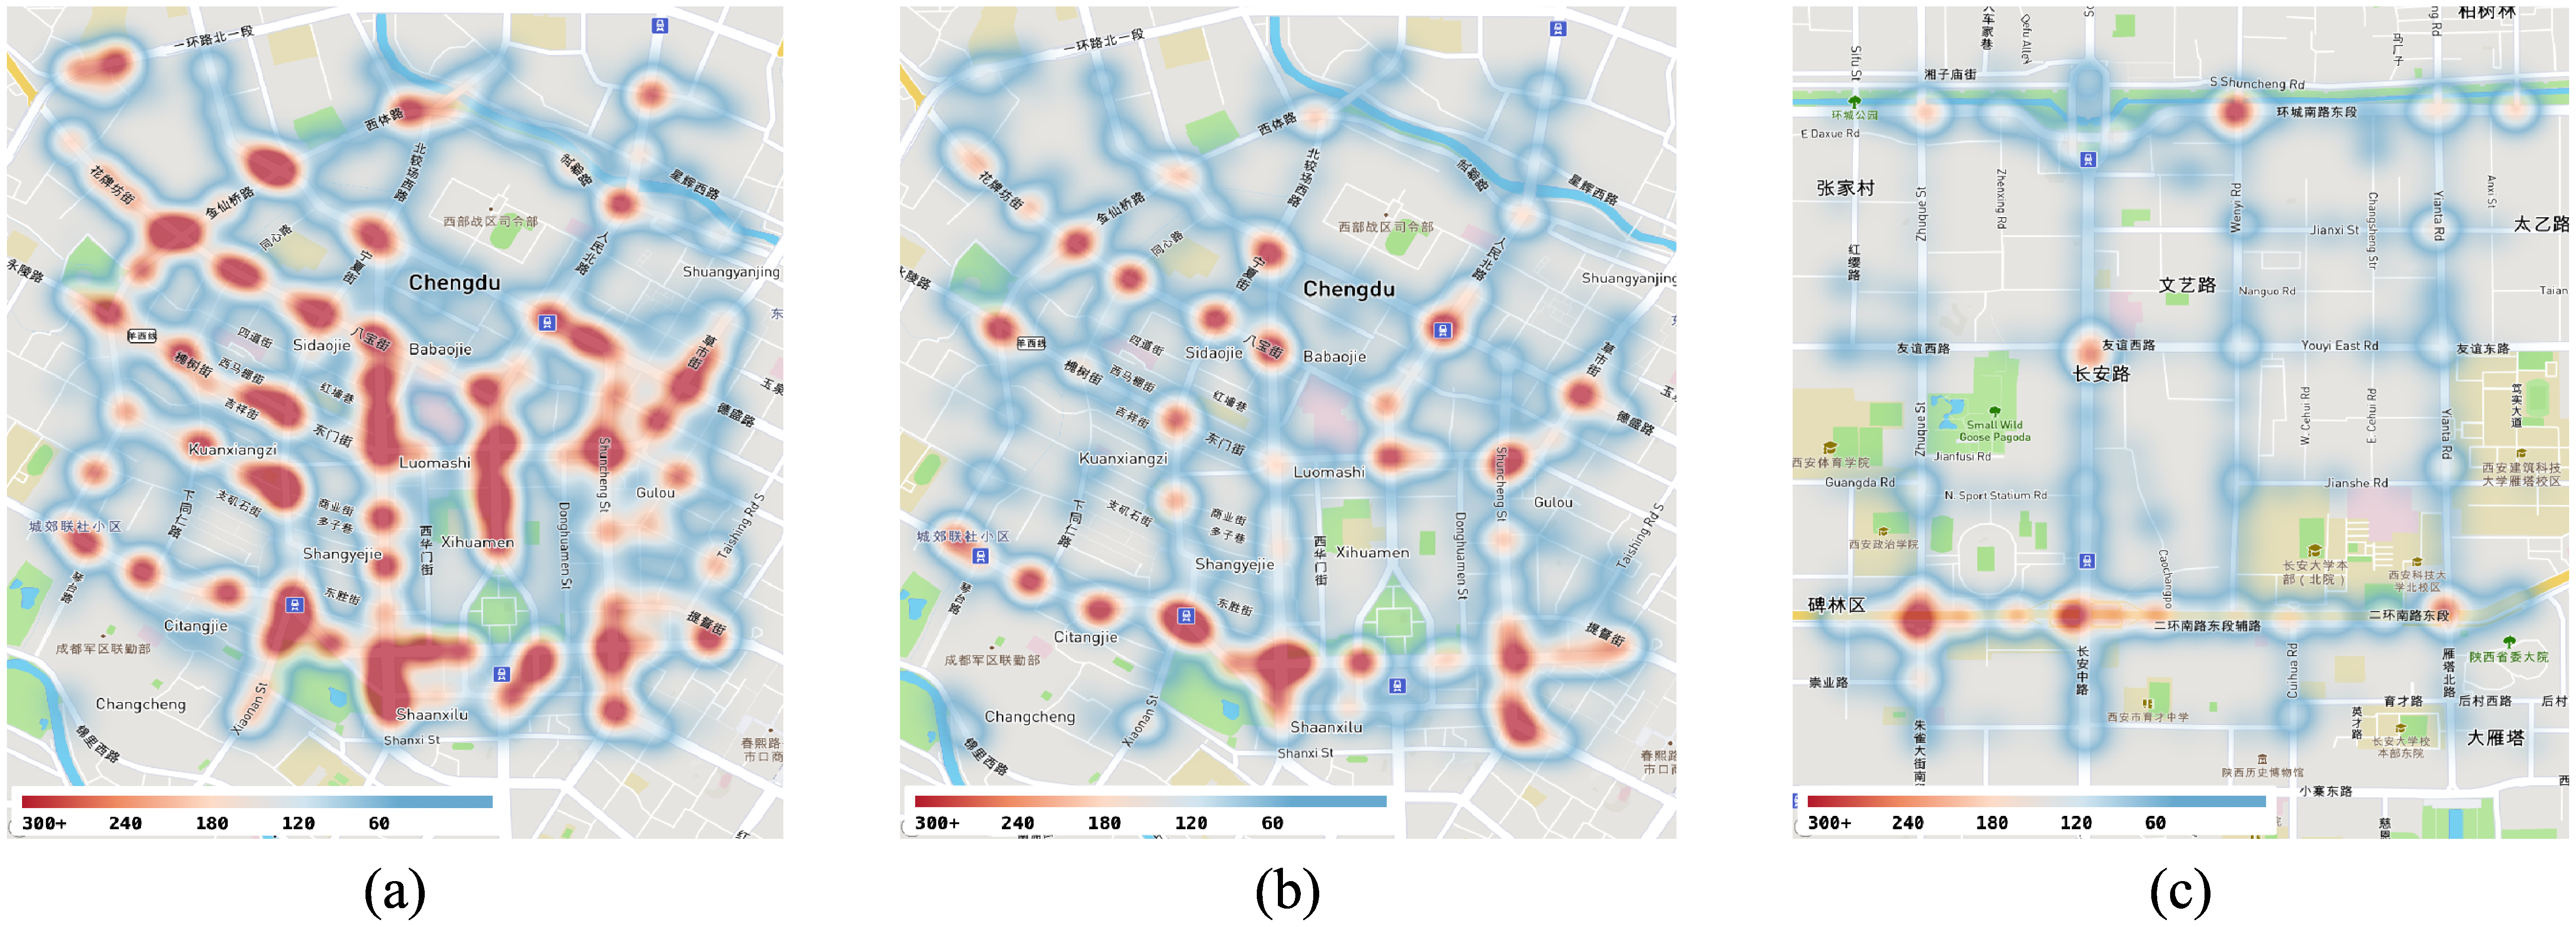
\includegraphics[width=1\columnwidth]{Fig3-4-heat-map.pdf}
  \bicaption[不同场景下的车辆分布热力图]{不同场景下的车辆分布热力图。(a) 场景1(b)场景2(c)场景3}[Heat map of the distribution of vehicles under different scenarios]{Heat map of the distribution of vehicles under different scenarios. (a) Scenario 1 (b) Scenario 2 (c) Scenario 3}
  \label{fig 3-4}
\end{figure} 

为了实现MDR,我们使用以下架构和超参数:
本地行动者网络是一个四层全连接的神经网络,其中包括两个隐藏层,神经元数量分别为64和32。
目标行动者网络的结构与本地行动者网络相同。
本地评论家网络是一个四层全连接的神经网络,其中包括两个隐藏层,神经元数量分别为128和64。
目标评论家网络的结构与本地评论家网络相同。
使用整流线性单元(Rectified Linear Unit,简称ReLU)作为激活函数,使用自适应矩估计(Adaptive Moment Estimation,简称 Adam)优化器更新网络权重,学习率为0.001,折扣系数设置为0.996。
经验回放缓冲区$|\mathcal{B}|$的大小被设置为100000,最小批量$M$的大小被设置为512。
此外,我们还实现了以下四种可比较的算法:

\begin{itemize}
	\item \textbf{随机分配}(Random Allocation,简称RA): 在每个时间片中,随机选择一个关于确定感知频率、上传优先级和V2I带宽分配的动作。
	\item \textbf{集中式深度确定性策略梯度}(Centralized Deep Deterministic Policy Gradient,C-DDPG) \cite{mlika2022deep}: 在边缘节点实现一个智能体,根据系统状态以集中的方式确定感知频率、上传优先级和V2I带宽分配。同时,智能体接收系统奖励以评估其贡献。
	\item \textbf{多智能体行动者-评论家}(Multi-Agent Actor-Critic,MAAC) \cite{he2021efficient}: 实现了车辆中的智能体,基于本地车联网环境观测来决定感知频率和上传优先级,以及边缘节点中的智能体来决定V2I带宽分配。每个智能体都接收系统奖励,以评估其贡献,这对每个智能体都是相同的。
	\item \textbf{利用VBA策略进行带宽分配的MAAC}(MAAC-VBA): 为了更好地分配V2I带宽,本章进一步设计了一个名为MAAC-VBA的变体,其中边缘节点根据预测的车辆轨迹和视图要求来分配V2I带宽。
\end{itemize}

此外,本章还设计了以下指标用于性能评估。
\begin{itemize}
	\item \textbf{累积奖励} (Cumulative Reward,简称CR): 定义为调度期间的累积系统奖励, 其计算方法为
		\begin{equation}
			\operatorname{CR} = \sum_{\forall t \in \mathbf{T}} r\left(\boldsymbol{a}_{v}^{t},\boldsymbol{a}_{e}^{t} \mid \boldsymbol{o}^{t}\right)
		\end{equation}
	\item \textbf{平均奖励的构成} (Composition of Average Reward,简称CAR): 定义为归一化的及时性、完整性和一致性在平均奖励中的百分比,其表示为
		\begin{equation}
			\operatorname{CAR} = <\frac{3}{10}(1-\hat{\Xi}_{i}),\frac{4}{10}(1-\hat{\Phi}_{i}), \frac{3}{10}(1-\hat{\Psi}_{i})>
		\end{equation}
	\item \textbf{平均排队时间} (Average Queuing Time,简称 AQT): 定义为感知信息的排队时间之和除以调度期$T$内的信息数量,其计算方法为 
		\begin{equation}
			\operatorname{AQT} =\sum_{\forall t \in \mathbf{T}} \left \{ \frac{\sum_{v \in \mathbf{V}} \sum_{\forall d \subseteq \mathbf{D}_{v}^t} \frac{\operatorname{q}_{d, v}^t}{|\mathbf{D}_{v}^t|} }{V} \right\} \bigg/ T
		\end{equation}
	\item \textbf{服务率} (Service Ratio,简称SR): 定义为满足完整性要求的视图的数量与调度期间$T$所需的视图总数的比率,其计算方法是 
		\begin{equation}
			\operatorname{SR} = \frac{\sum_{\forall t \in \mathbf{T}}\sum_{\forall i \in \mathbf{I}_e^t} \mathds{1}\{\Phi_{i} \geq \Phi_{threshold}\}}{ \sum_{\forall t \in \mathbf{T}} |\mathbf{I}_e^t|}
		\end{equation}
	其中 $\Phi_{threshold}$ 是完整性阈值。
\end{itemize}

\subsection{实验结果与分析}
\begin{figure}[h]
\centering
  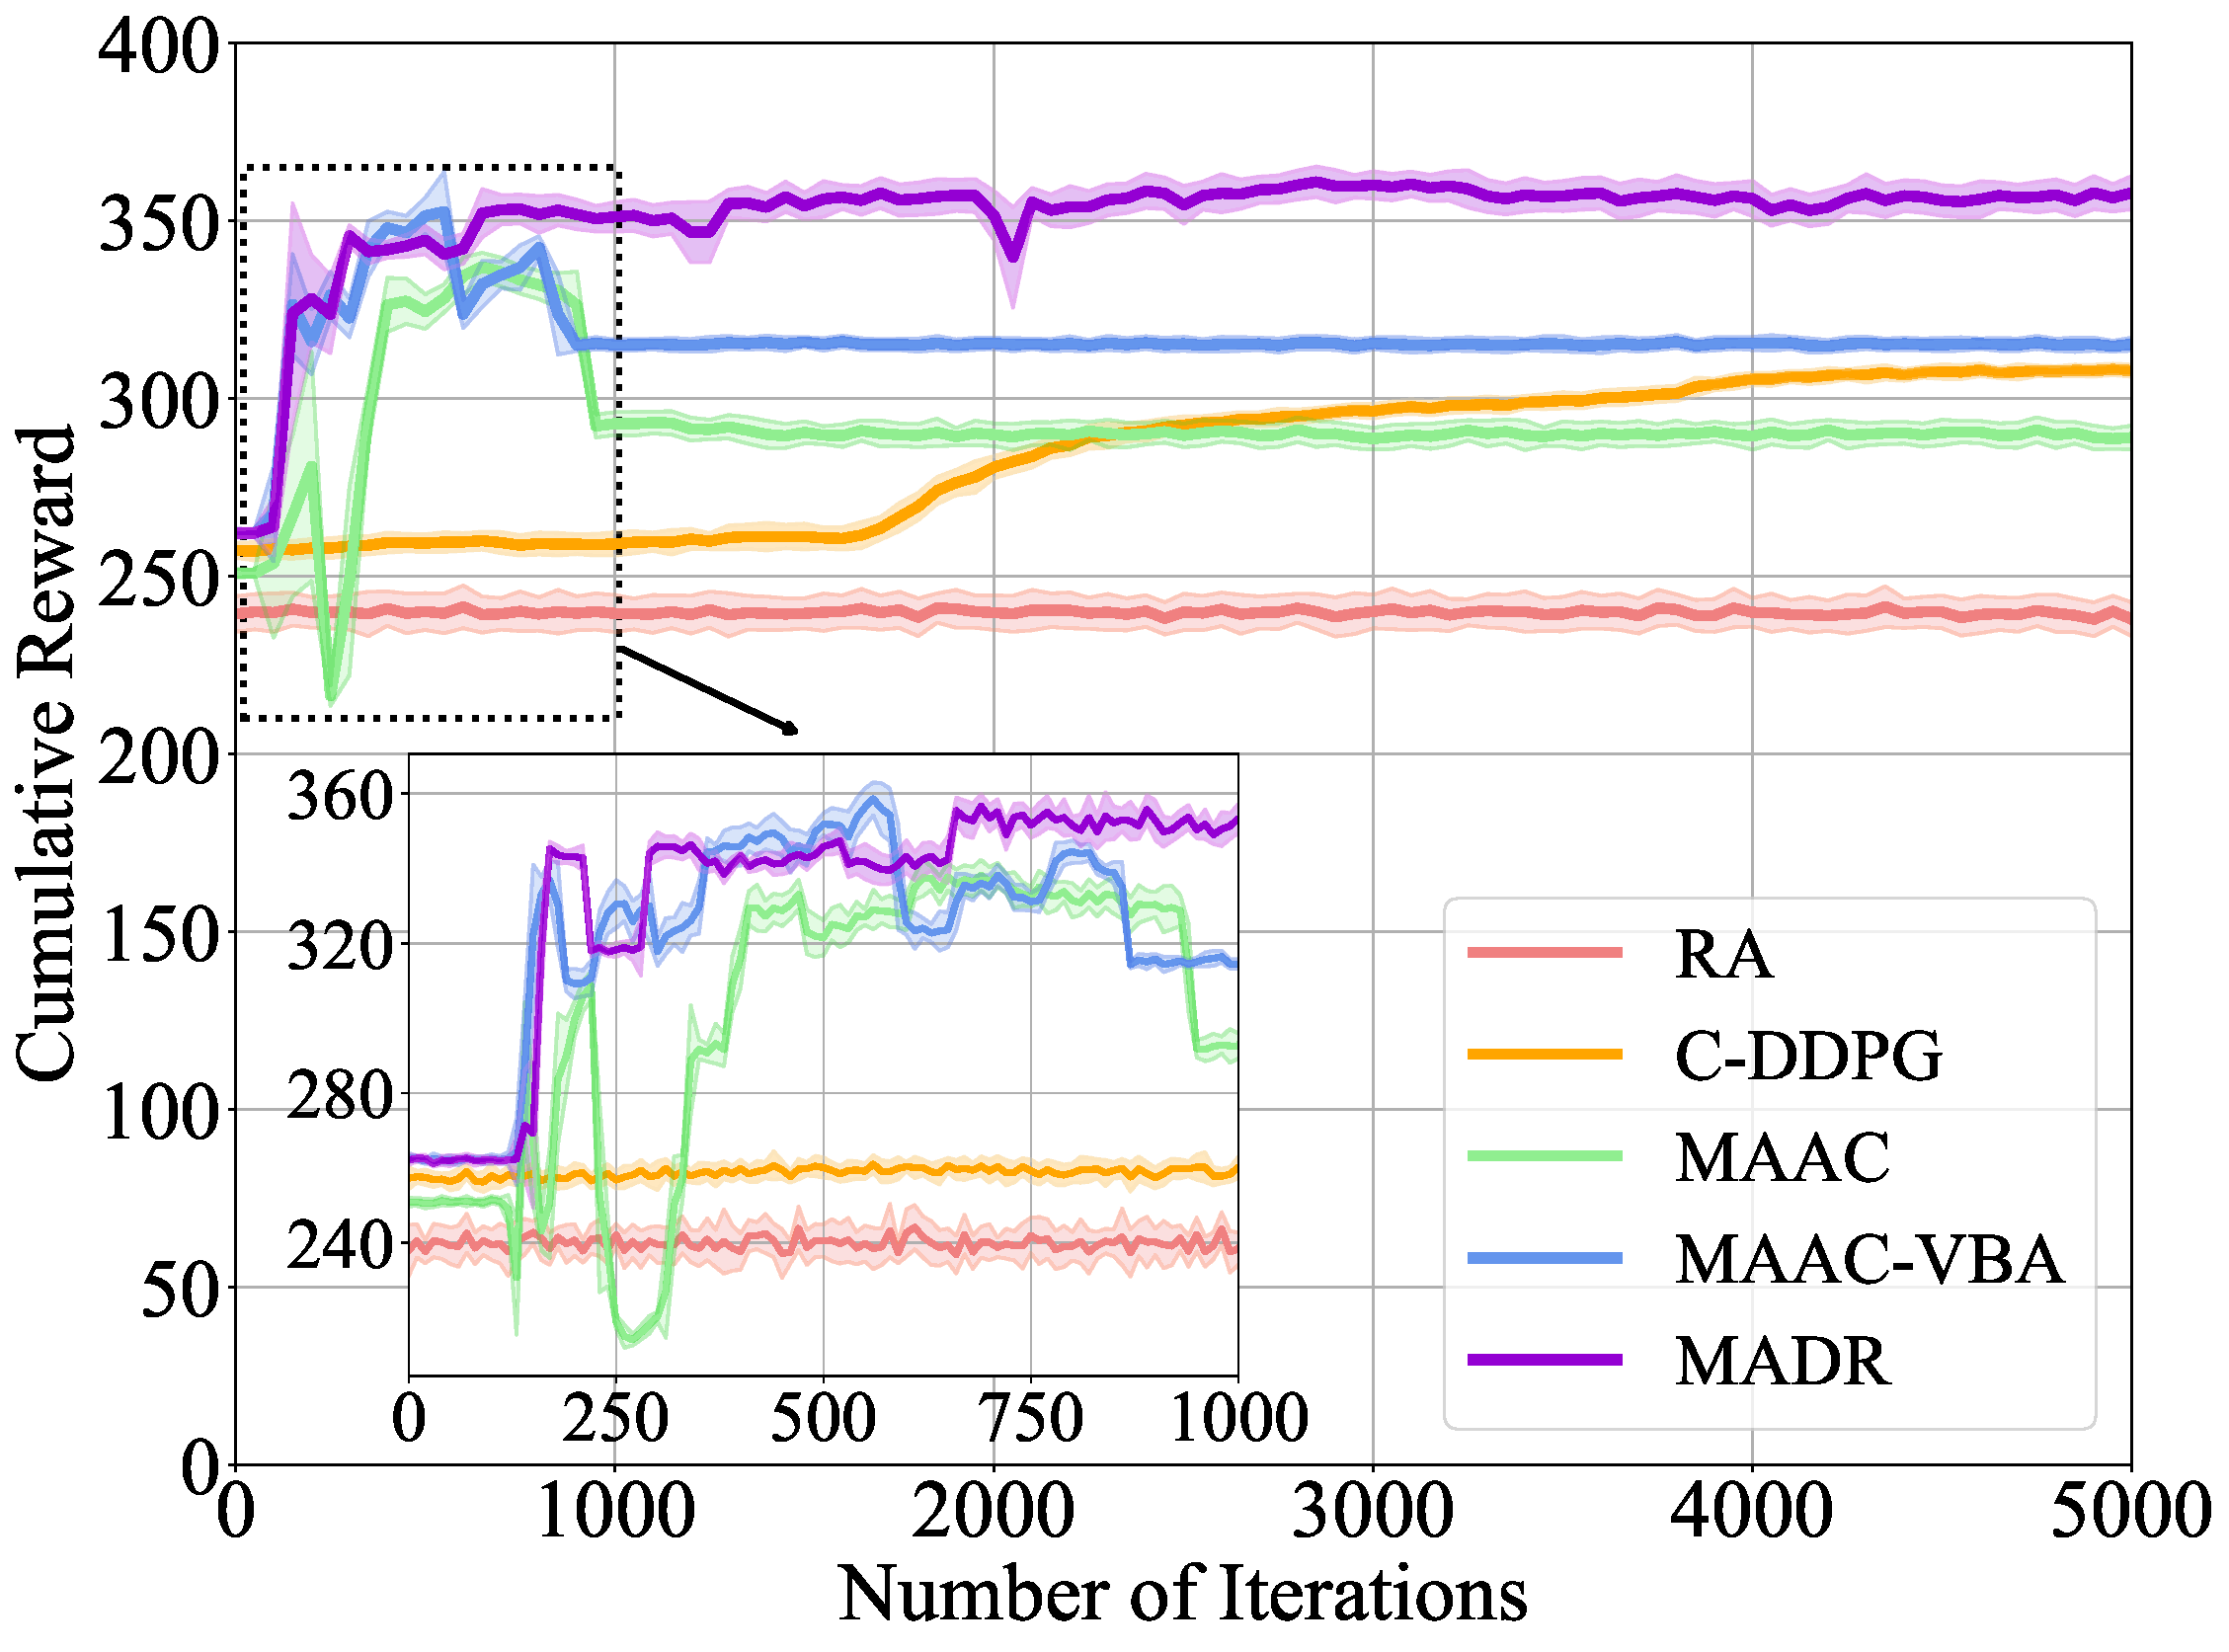
\includegraphics[width=1\columnwidth]{Fig3-5-convergence.pdf}
  \bicaption{算法收敛性比较}{Convergence comparison}
  \label{fig 3-5}
\end{figure} 

\textbf{1) 算法收敛性:}
图\ref{fig 3-5}比较了五种算法的收敛数据以及达到的CR值。
结果显示,本章提出的MDR算法具有最快的收敛速度(约660次迭代),并获得了最高的CR值(约357)。
相比之下,C-DDPG、MAAC和MAAC-VBA分别在大约4500次、950次和870次迭代后收敛,并分别达到约307、290和315的CR值。
RA作为基线算法实现了约241的CR值。
值得注意的是,与C-DDPG、MAAC和MAAC-VBA相比,MDR算法在CR值方面分别实现了大约16.3\%、23.1\%和13.3\%的增加,并在收敛速度方面分别有大约6.8倍、1.4倍和1.3倍的提升。
主要的原因是,所提MDR算法旨在维护车辆的稳定通信环境,这使得车辆中的行动者和评论家网络的训练更加有效。
另一方面,由于MDR的行动空间较小,因此相比于C-DDPG,MDR更容易收敛,因为C-DDPG使用DDPG智能体同时决定关于确定感知频率、上传优先级和V2I带宽分配的动作。

\begin{figure}[h]
  \centering
  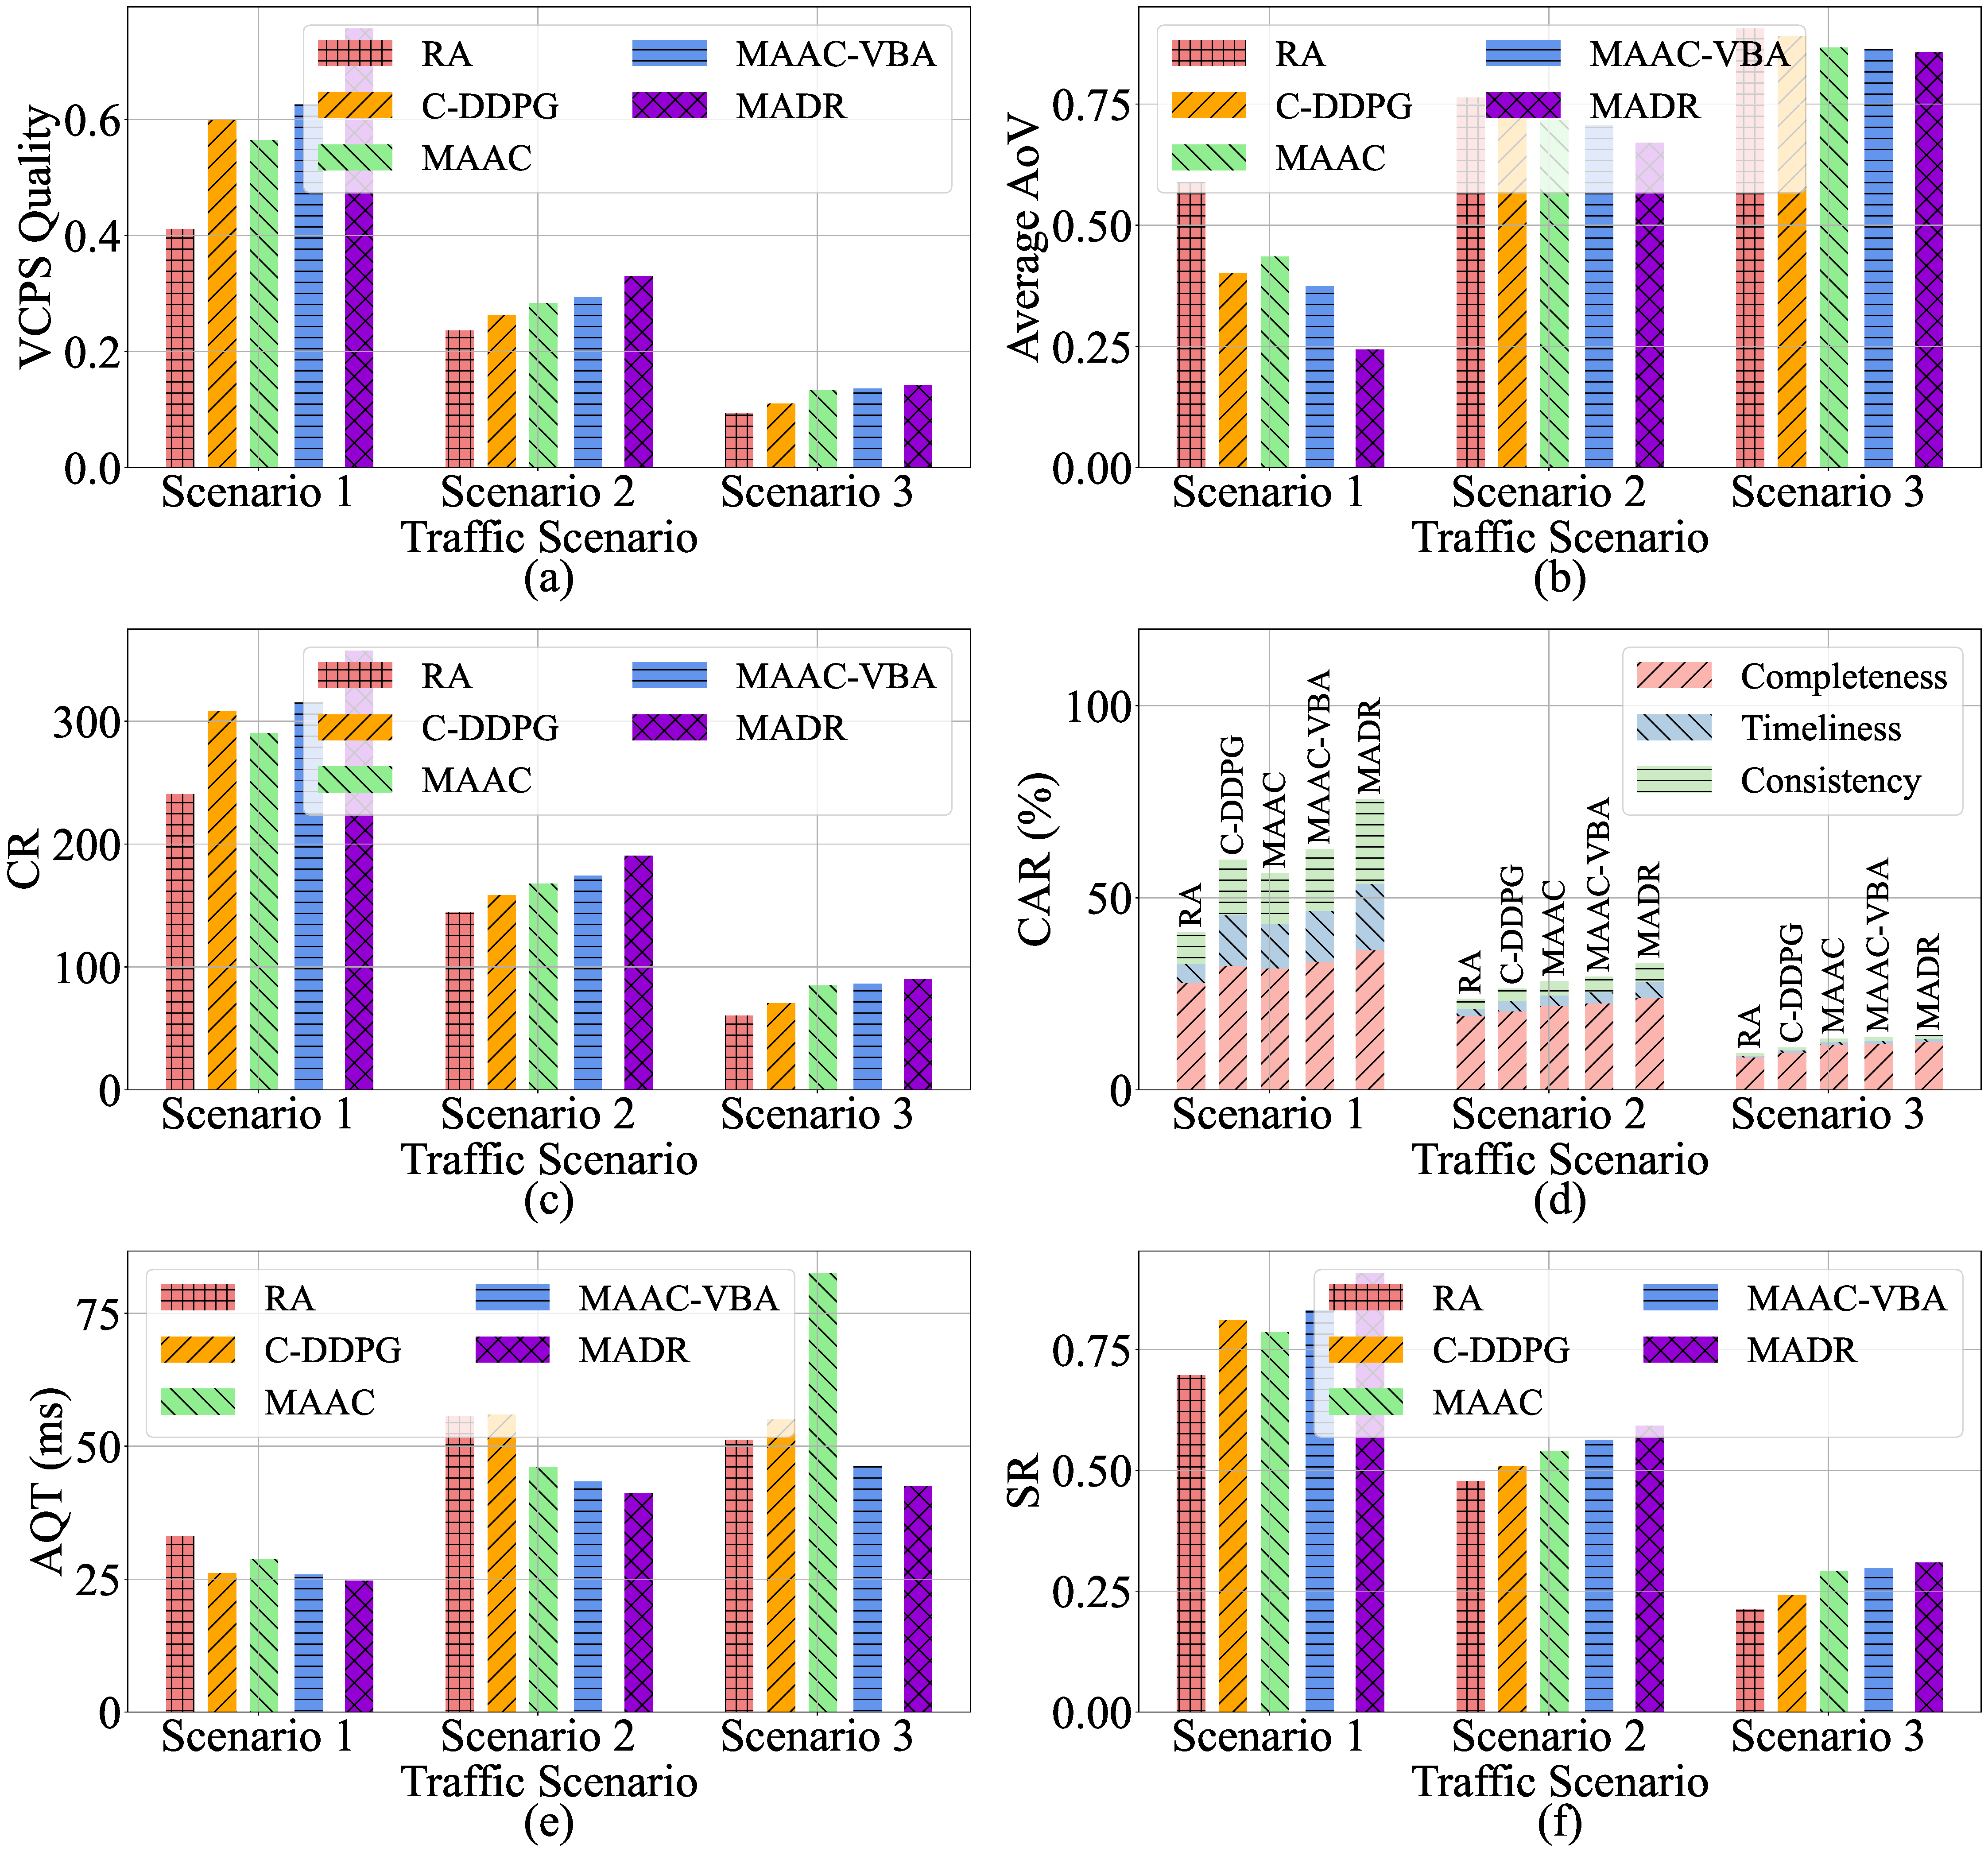
\includegraphics[width=1\columnwidth]{Fig3-6-different-scenarios.pdf}
  \bicaption[不同交通场景下的性能比较]{不同交通场景下的性能比较。(a)车载信息物理融合系统质量(b)平均 AoV(c)累积奖励(d)平均奖励的构成(e)平均排队时间(f)服务率}[Performance comparison under different traffic scenarios]{Performance comparison under different traffic scenarios. (a) Vehicular cyber-physical system quality (b) Average age of view (c) Cumulative reward (d) Composition of average reward (e) Average queuing time (f) Service ratio}
  \label{fig 3-6}
\end{figure}

\textbf{2) 交通场景的影响:}
图\ref{fig 3-6}比较了五种算法在不同交通场景下的性能。
图\ref{fig 3-6}(a)比较了五种算法的VCPS质量。
如图所示,所提MDR算法在所有场景下都能达到最高的VCPS质量。
特别是,在不同的交通场景下,MDR比RA、C-DDPG、MAAC和MAAC-VBA分别平均提高了58.0\%、27.1\%、19.1\%和12.5\%的VCPS质量。
图\ref{fig 3-6}(b)显示了五种算法的平均AoV。
与预想的一致,在所有场景下,MDR都能实现最低的平均AoV。
图\ref{fig 3-6}(c)比较了五种算法的CR。
如图所示,MDR实现的CR高于RA、C-DDPG、MAAC和MAAC-VBA。
同时,在场景3下,MDR和MAAC-VBA的CR是相似的。
原因是场景3中较低的车辆密度和较高的车辆动态性使得数据上传比场景1和2中更困难。

图\ref{fig 3-6}(d)将平均奖励分成三部分,分别显示了及时性、完整性和一致性的比例。
可以看出,在场景3下,五种算法的及时性和一致性都非常小。
这主要是因为当视图不完整时,及时性和一致性的要求很难得到满足。
图\ref{fig 3-6}(e)和\ref{fig 3-6}(f)比较了不同交通场景下五种算法的AQT和SR。
它表明,MDR实现了最低的AQT,并在所有情况下保持最高的SR。

\begin{figure}[h]
  \centering
  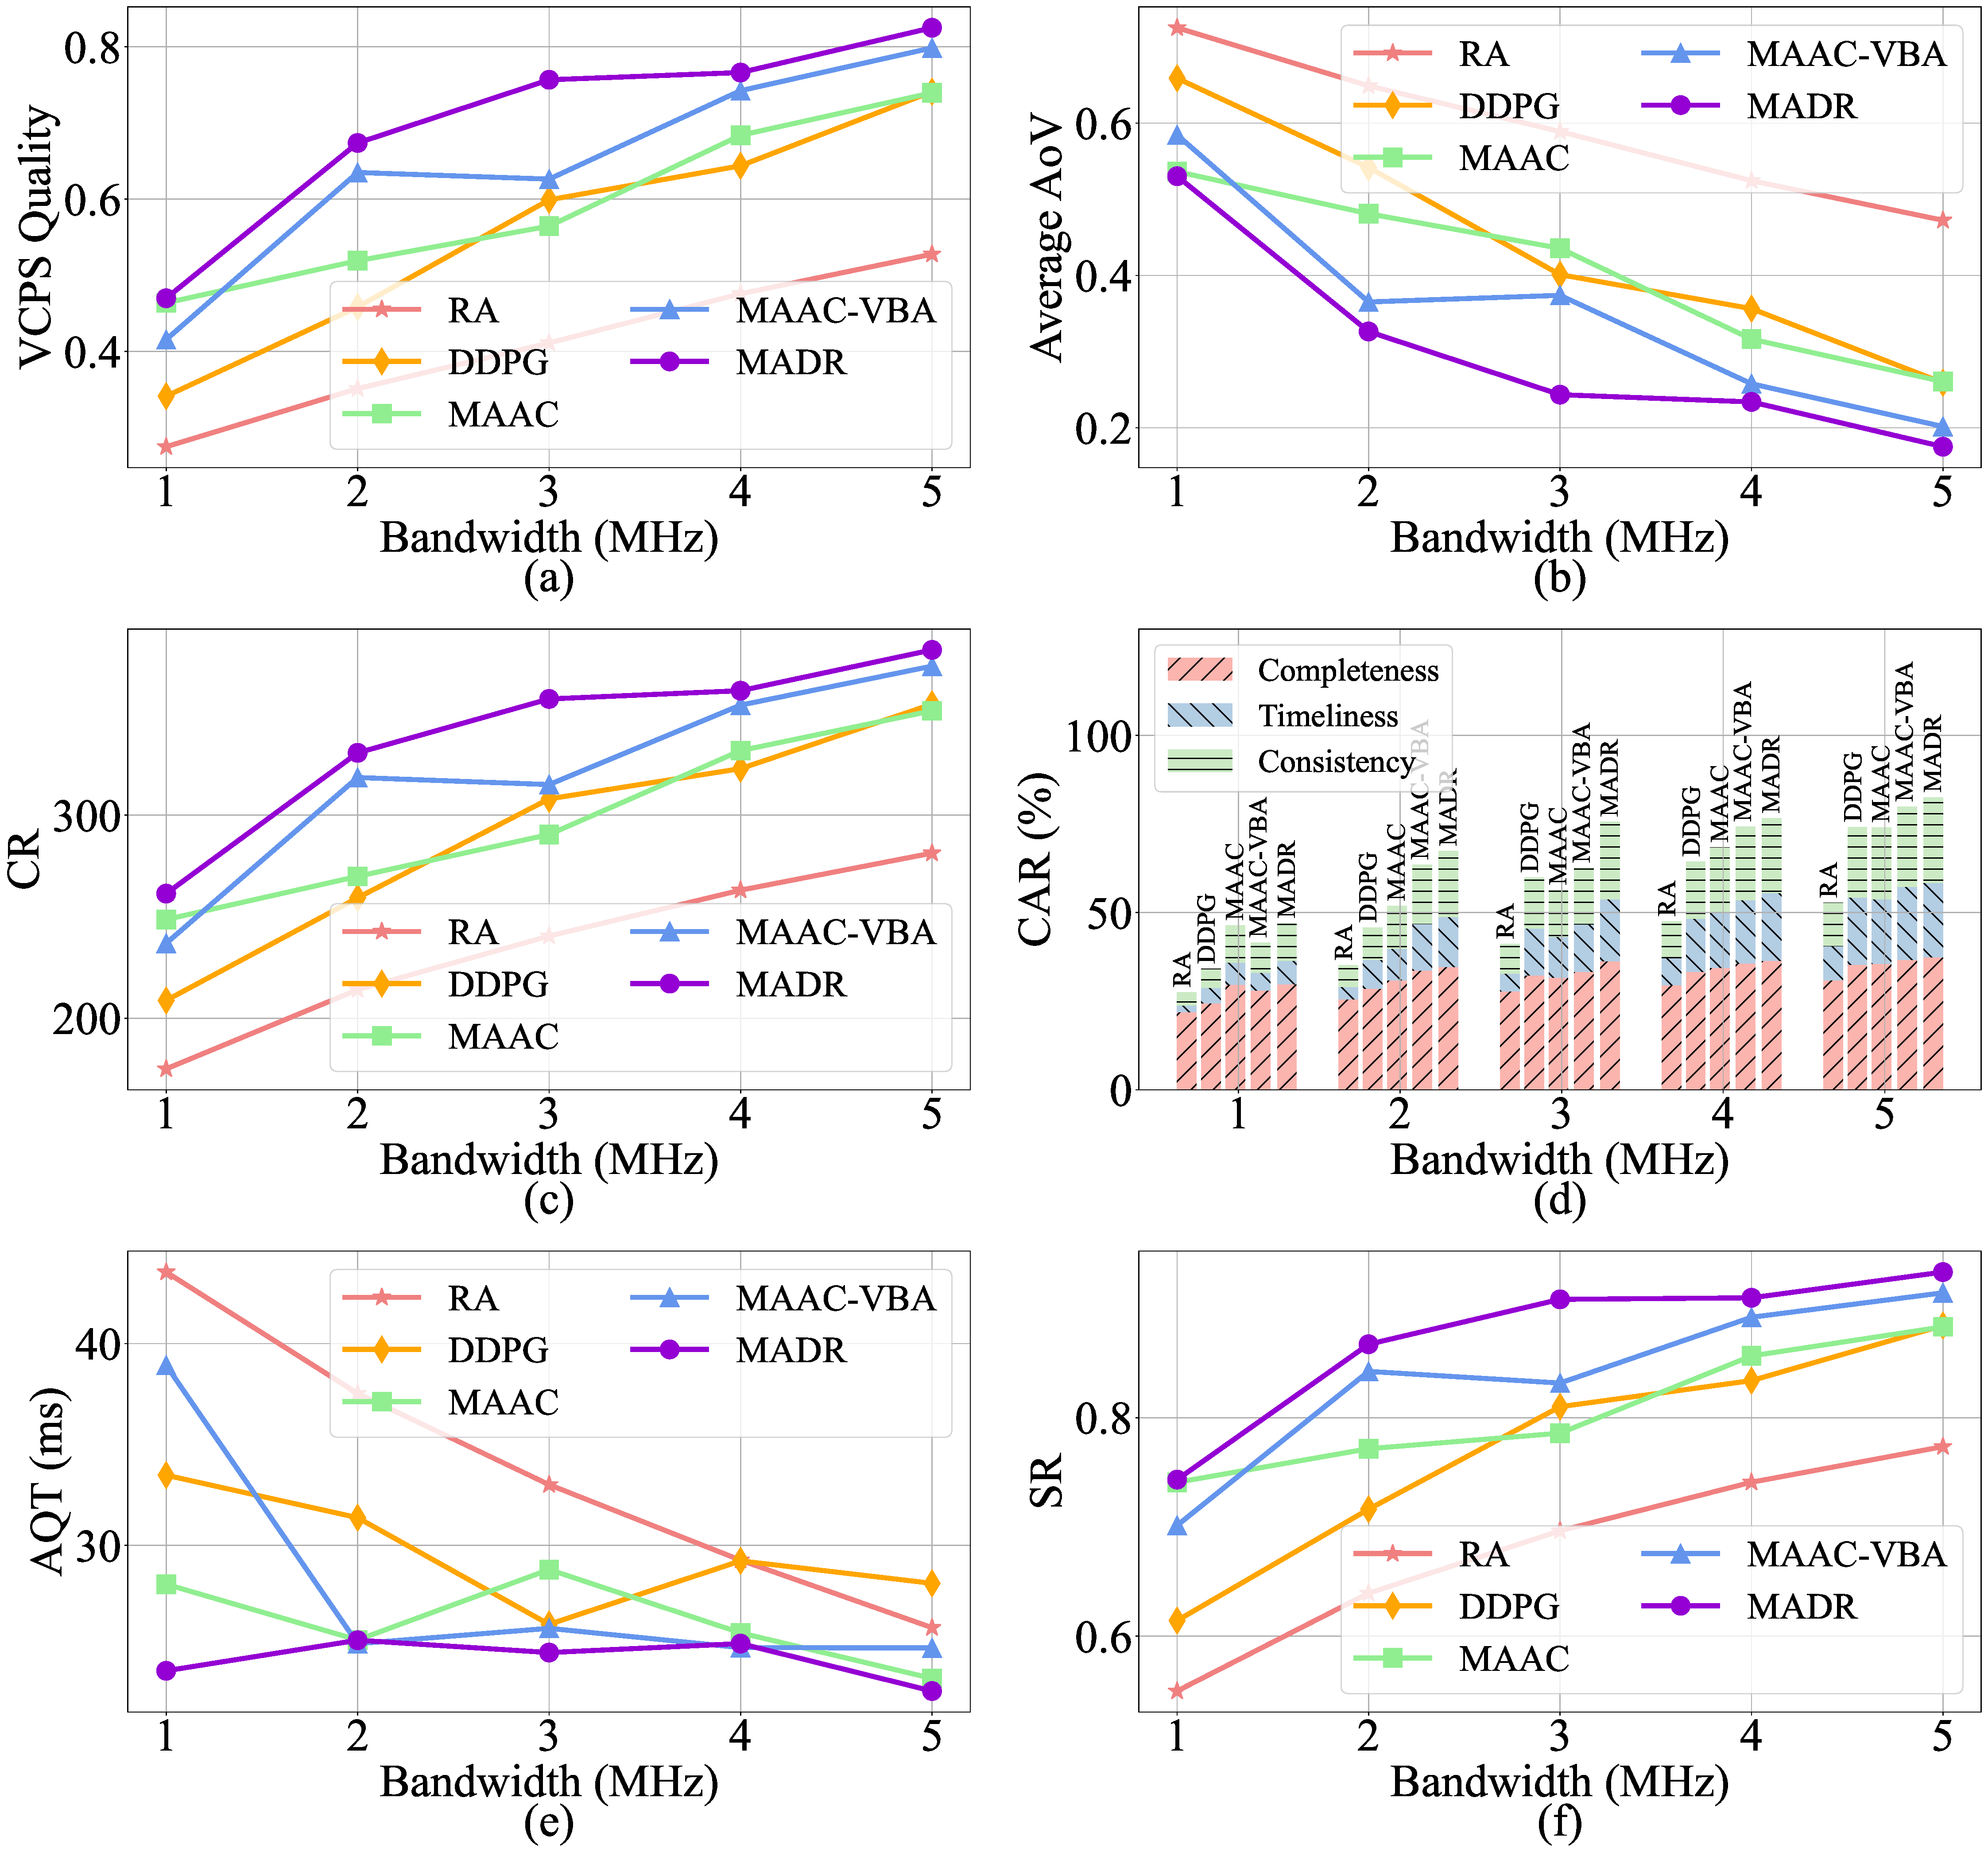
\includegraphics[width=1\columnwidth]{Fig3-7-different-bandwidths.pdf}
  \bicaption[不同V2I带宽下的性能比较]{不同V2I带宽下的性能比较。(a)车载信息物理融合系统质量(b)平均 AoV(c)累积奖励(d)平均奖励的构成(e)平均排队时间(f)服务率}[Performance comparison under different V2I bandwidths]{Performance comparison under different V2I bandwidths. (a) Vehicular cyber-physical system quality (b) Average age of view (c) Cumulative reward (d) Composition of average reward (e) Average queuing time (f) Service ratio}
  \label{fig 3-7}
\end{figure}

\textbf{3) V2I 带宽的影响:}
图\ref{fig 3-7}比较了不同V2I带宽下五种算法的性能。
在这组实验中,边缘节点的V2I带宽从1MHz增加到5MHz。
更大的带宽代表更多的信息可以通过V2I通信上传。
图\ref{fig 3-7}(a)比较了五种算法的VCPS质量。
随着带宽的增加,所有算法的VCPS质量都相应增加。
在边缘节点的不同带宽下,MDR的VCPS质量分别比RA、C-DDPG、MAAC和MAAC-VBA高出约72.9\%、28.3\%、17.8\%和9.3\%。
图\ref{fig 3-7}(b)比较了这五种算法的平均AoV。
特别是,MDR在所有情况下实现了最低的平均AoV。
图\ref{fig 3-7}(c)比较了五种算法的CR。
正如预期的那样,当带宽增加时,所有五种算法的性能都会变好。
具体来说,与RA、C-DDPG、MAAC和MAAC-VBA相比,MDR在CR方面分别实现了75.1\%、29.4\%、22.7\%和10.6\%的提升。

图\ref{fig 3-7}(d) 比较了五种算法的CAR。
MDR比其他四种算法取得了更好的性能,特别是在及时性和平均奖励的一致性方面。
这是因为在有限的带宽下,所提出的方案中车辆之间的信息感知和上传的协作更加有效。
图\ref{fig 3-7}(e) 比较了五种算法的AQT。
如图所示,在不同的V2I带宽下,MDR的AQT保持最低,这反映了所设计的MDR能够更有效地分配带宽。
图\ref{fig 3-7}(f)显示了五种算法的SR,可以进一步证明这一优势。
在所有情况下,MDR的SR都保持在最高水平。


\begin{figure}[h]
  \centering
  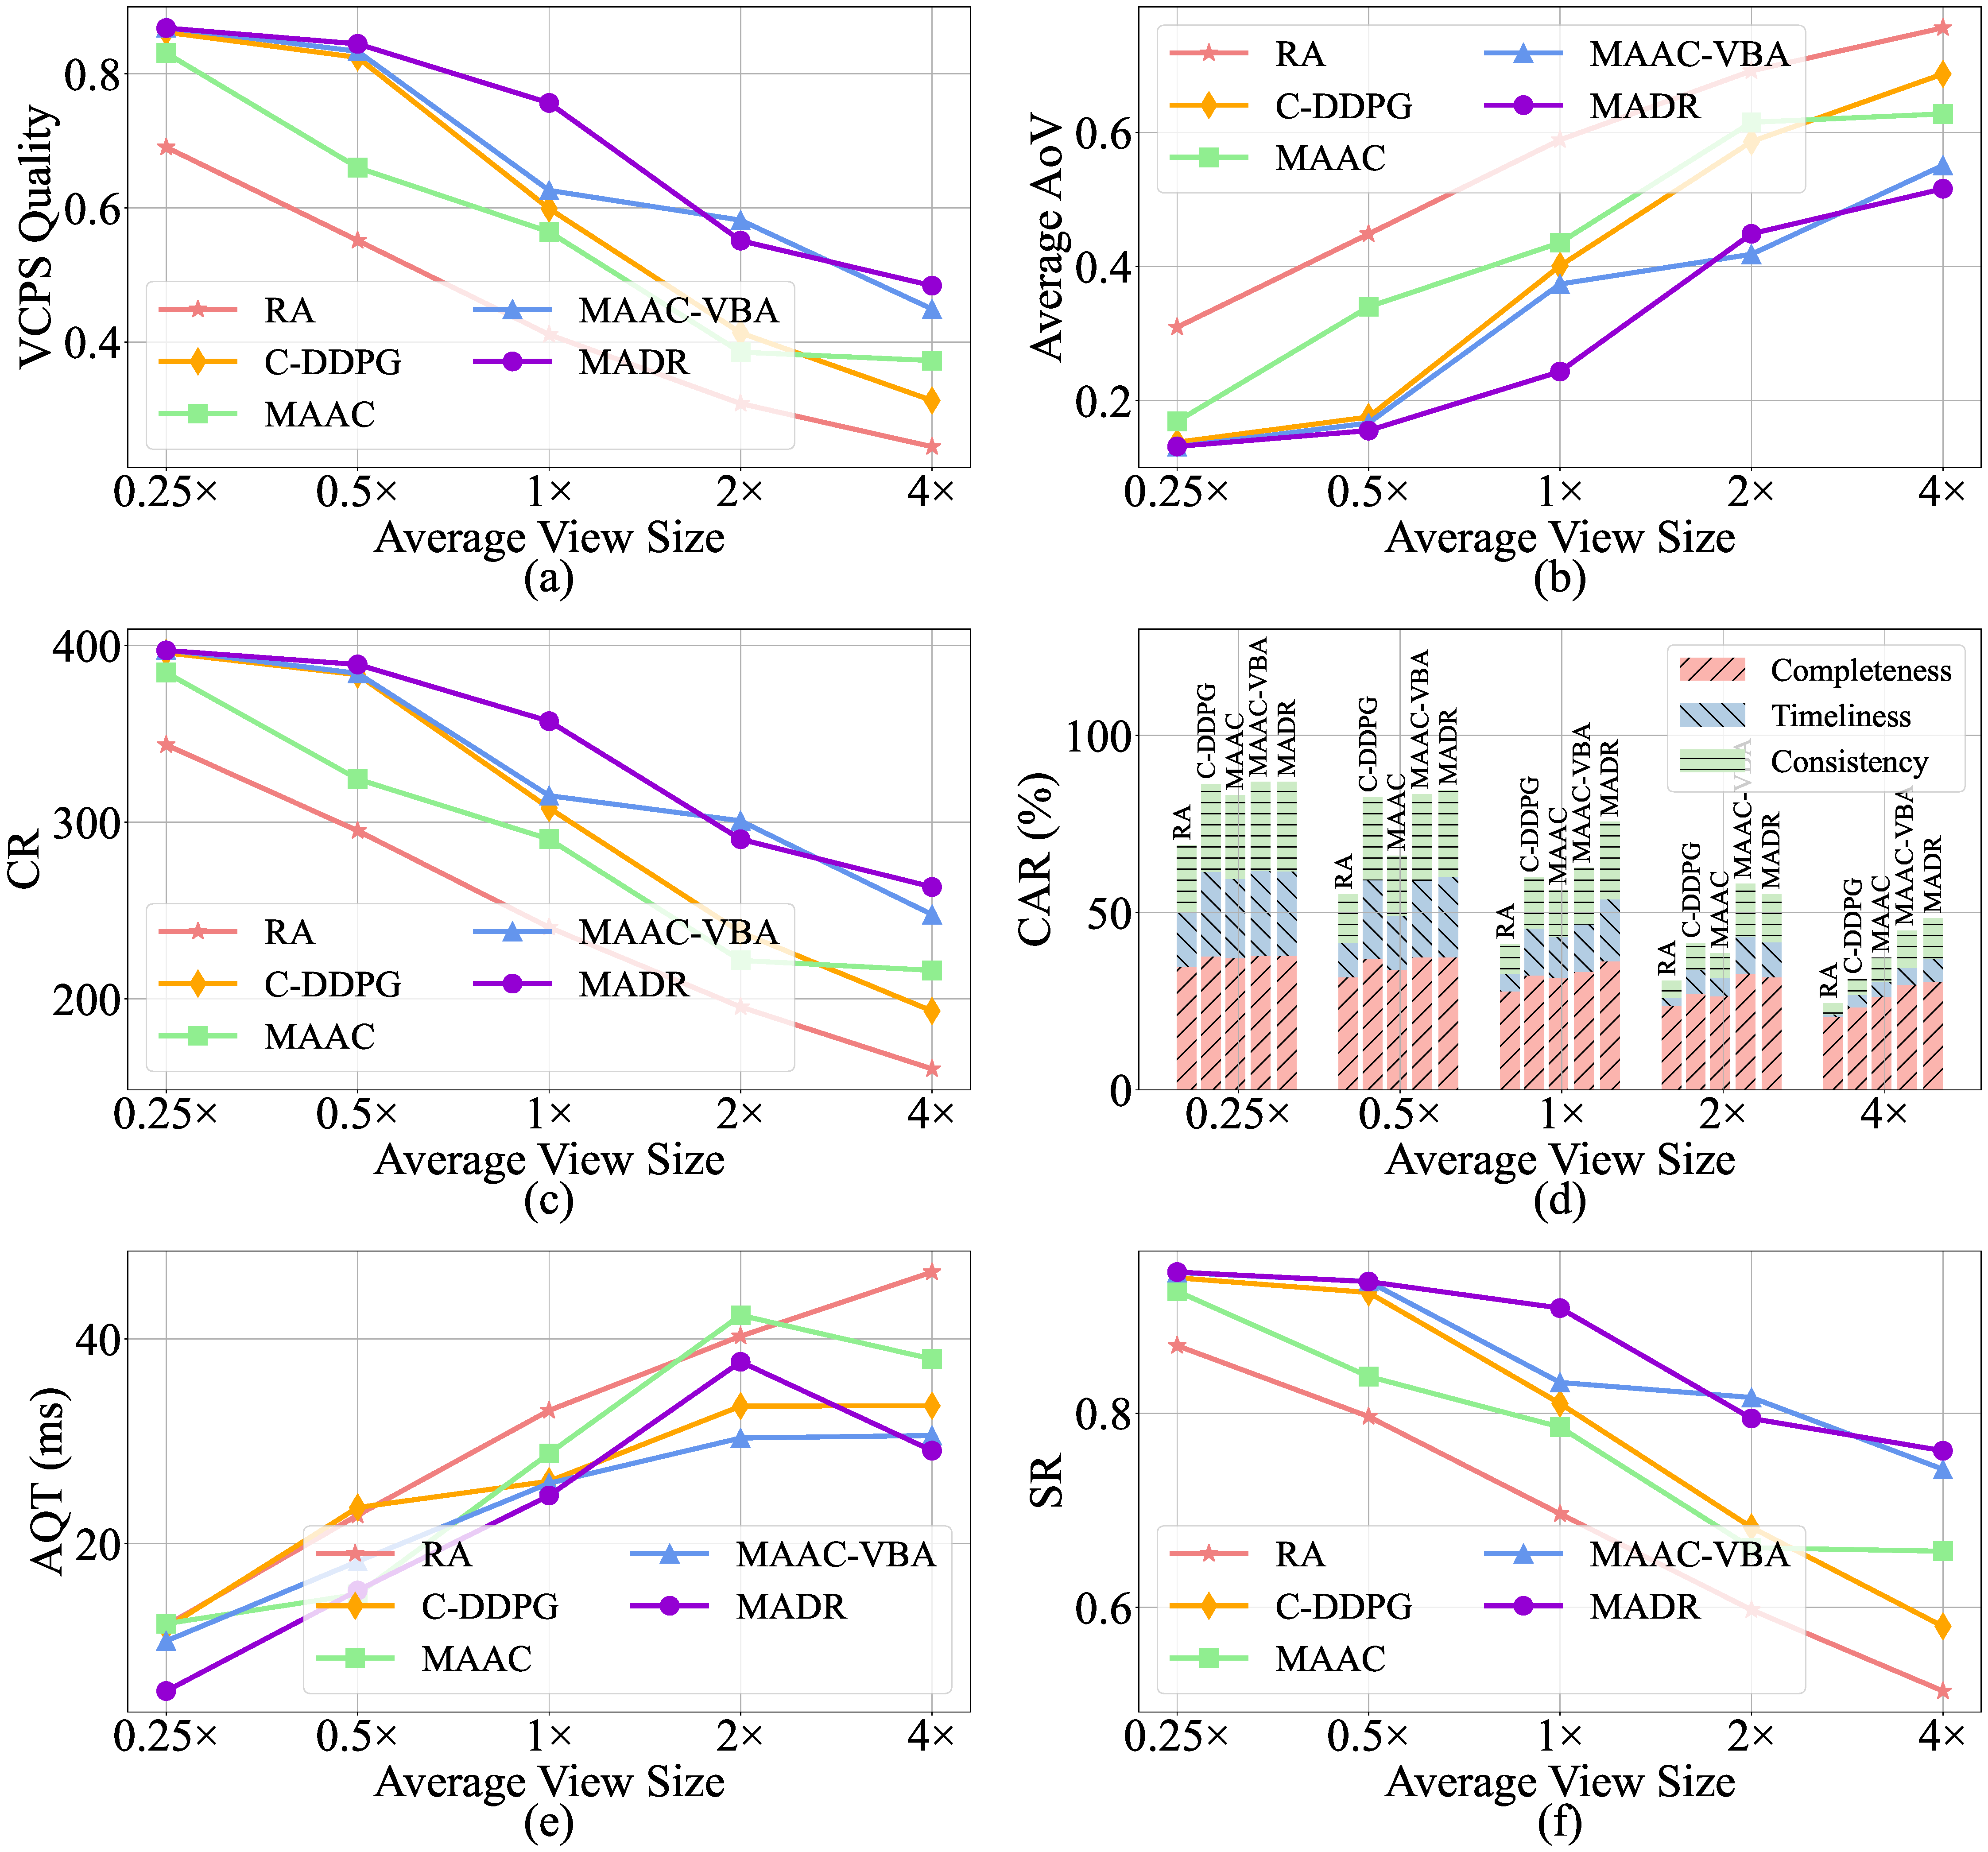
\includegraphics[width=1\columnwidth]{Fig3-8-different-view-sizes.pdf}
  \bicaption[不同视图需求下的性能比较]{不同视图需求下的性能比较。(a)车载信息物理融合系统质量(b)平均 AoV(c)累积奖励(d)平均奖励的构成(e)平均排队时间(f)服务率}[Performance comparison under different requirements on views]{Performance comparison under different requirements on views. (a) Vehicular cyber-physical system quality (b) Average age of view (c) Cumulative reward (d) Composition of average reward (e) Average queuing time (f) Service ratio}
  \label{fig 3-8}
\end{figure}

\textbf{4) 视图需求的影响:}
图\ref{fig 3-8}比较了五种算法在对视图的不同需求下的性能,其中ITS应用需求的视图平均大小从0.25倍增加到4倍,1倍的平均视图大小约为6.46MB。
图\ref{fig 3-8}(a)比较了五种算法的VCPS质量。
正如预期的那样,当平均视图大小增加时,五种算法的性能都会变差。
在不同的视图应用要求下,MDR在最大限度地提高VCPS质量方面分别比RA、C-DDPG、MAAC和MAAC-VBA高出约68.1\%、23.5\%、27.9\% 和4.9\%。
图\ref{fig 3-8}(b)和\ref{fig 3-8}(c)比较了五种算法的平均AoV和CR。
当平均视图大小较小时(即1.62MB左右),MDR中的平均AoV略低于MAAC和MAAC-VBA。
同时,值得注意的是,MDR、MAAC和MAAC-VBA的CR是相似的。
原因是较小的数据量有较高的成功上传的概率。

图\ref{fig 3-8}(d)比较了五种算法的CAR。
可以看出,当平均视图大小从0.25倍增加到0.5倍时,MDR和MAAC-VBA之间的性能差异很小。
原因是当有足够的资源来满足较小的平均视图大小(即1.62MB和3.23MB左右)的要求时,算法的调度效果并不明显。
图\ref{fig 3-8}(e)和\ref{fig 3-8}(f)比较了五种算法的AQT和SR,表明MDR可以保持最低的AQT,同时在大多数情况下实现最高的SR。
值得注意的是,当平均视图大小为2倍时,MAAC-VBA实现了最低的AQT和最高的SR,这反映了所提出的VBA方案可以更有效地分配带宽。

\section{本章小结}\label{section 3-6}

本章提出了一种新的指标AoV,用于评估边缘构建的逻辑视图,即车载信息物理融合中异质信息的质量,包括及时性、完整性和一致性。
在此基础上,提出了最大化VCPS质量的问题,并设计了一个基于多智能体强化学习的解决方案,其中车辆作为独立智能体,决定感知频率和上传优先级。
边缘节点通过考虑车辆轨迹和视图要求,基于VBA策略分配V2I带宽。
并采用基于DR的信用分配方案,根据车辆个人贡献评估奖励。
通过仿真实验的全面性能评估表明,所提MDR算法比RA、C-DDPG、MAAC和MAAC-VBA在最大限度地提高VCPS质量方面分别高出约61.8\%、23.8\%、22.0\%和8.0\%,同时加快了收敛速度。

